\DocumentMetadata{} % lualatex + this line = bookmark content page error
\InputIfFileExists{zlatex_l3doc-cfg.tex}{}{}
\documentclass[
  lang=cn, 
  hyper=true,
  class=l3doc, 
  % classOption={show-notes}
  % layout={slide, aspect=16|9, theme=AnnArborSpruce}
]{../code/zlatex}
\usepackage{ztool}
\zlatexloadlibrary{mathalias}
\zlatexloadlibrary{theme}
\zlatexSetup{
  toc={
    column=2,
    title=\hfill\large\normalfont CONTENTS {\sffamily\small NEW}\hfill,
    stretch=1.3
  }
}
\zlatexColorSetup{
  link=purple
}
\geometry{left=2in, right=1in}
\usepackage{zhnumber}
\usepackage{tikzlings}
\usepackage{booktabs}
\usepackage{comment}
\usepackage{tabularray}
\UseTblrLibrary{diagbox}
\usepackage{pifont}
\usepackage{pdfpages}
\usepackage{multicol}
\usepackage{hologo}
\usepackage{minted}
\usepackage[bottom]{footmisc}
\usepackage{transparent}
\fvset{gobble=0}
\setmonofont{Latin Modern Mono}[
  BoldFont=*,
  ItalicFont=* Slanted,
  BoldItalicFont=* Slanted,
  BoldFeatures={FakeBold=2},
  BoldItalicFeatures={FakeBold=2},
]
\newfontfamily{\russia}[Path=./support/Fonts/]{cmunrm.ttf}[
  BoldFont=cmunbx.ttf,
  ItalicFont=cmunbi.ttf
]
\ExplSyntaxOn
\newcommand{\zkey}[1]{
  \clist_clear:N \l_tmpa_clist
  \clist_map_inline:nn {#1}{
    \clist_put_right:Nn \l_tmpa_clist {\meta{##1}}
  }
  \clist_use:Nn \l_tmpa_clist {,~}
}
\ExplSyntaxOff
\newcommand{\block}[1]{{\color{#1}\rule{1em}{1em}}}
\newcommand{\Footnote}[1]{\stepcounter{footnote}\footnote[\thefootnote]{#1}}
\definecolor{slideRed}{HTML}{a30000}
\definecolor{slideGray}{HTML}{e0e0e0}
\definecolor{slideWhite}{HTML}{f0f0f0}
\definecolor{zchapColor}{HTML}{7f8184}
\definecolor{Ann-default-I}{HTML}{0000a3}
\definecolor{zslide@color@title}{HTML}{d9d9d9}
\colorlet{RoyalRed}{zlatex@color@royalred}
\definecolor{bg}{rgb}{0.95,0.95,0.95}
\setminted{
  bgcolor=bg,
  breaklines=true, 
  tabsize=2,
  breakanywhere=true,
  breaksymbolright=$\swarrow$,
  breakanywheresymbolpre=,
  breaksymbolleft=,
}
% \usepackage[most]{tcolorbox}
% \tcbuselibrary{listings, minted, breakable, skins}
\newcounter{DocExample}
\tcbuselibrary{minted}
\tcbset{listing engine=minted}
\DeclareTCBListing{DocExample}{!s!O{//}}{
  enhanced, 
  breakable,
  % frame hidden, arc=2pt,
  enhanced jigsaw,
  opacityback=0, 
  sharp corners, 
  colframe=black, boxrule=.4pt,
  left=.5mm, right=1mm,
  top=0mm, bottom=0mm, 
  \IfBooleanTF{#1} 
    {listing and text}
    {listing only},
  minted language=tex, 
  minted options = {  
    autogobble,
    escapeinside=#2,
    bgcolor=,
    fontsize=\small,
  },
  overlay unbroken and first = {
    \node[anchor=north east, outer sep=0pt, text=red] 
      at (frame.north east) { \stepcounter{DocExample}\textbf{例\ \theDocExample}};
  }
}
\newcommand{\zlatex}{{}\lowercase{z}\LaTeX{}}
\newcommand{\zclassArg}{\textcolor{red}{\ding{73}}}
\newcommand{\zcmdArg}{\textcolor{red}{\(\star\)}}
\newcommand{\zFullExp}{\textcolor{red}{\(\star\)}}
\newcommand{\zResExp}{\textcolor{red}{\ding{73}}}
\NewDocumentCommand{\zdefault}{sm}{%
  \IfBooleanTF{#1}%
    {\textcolor{red}{\textbf{#2}}}%
    {\textcolor{red}{:\textbf{#2}}}%
}
\newcommand{\zarg}[1]{\texttt{\{}\cmd{#1}\texttt{\}}}


%%%%% Temp env or cmd declaration %%%%%
\usepackage{comment}
\def\blindText{As any dedicated reader can clearly see, the Ideal of practical
reason is a representation of, as far as I know, the things in themselves; 
\begin{align}
\underset{}{\mathbf{v} \bigotimes \mathbf{w}} 
    & = \sum_{i=1}^3\left(a_{i1}u^iv^1+a_{i2}u^iv^2+a_{i3}u^iv^3\right) \\
    & = \int x \dd x = \frac12 x^2 + \R{C} 
  \end{align}  
As any dedicated reader can clearly see, the Ideal of practical reason is a 
representation of, as far as I know, the things in themselves;}


\ExplSyntaxOn\makeatletter
\prop_new:N \g_arabix_suffix_prop
\prop_set_from_keyval:Nn \g_arabix_suffix_prop {
  1=st, 2=nd, 3=rd, 11=th, 12=th, 13=th, 0=th, _=th
} 
\NewDocumentCommand\zlatexNumSuffix{m}{
  \int_compare:nTF {11 <= #1 <= 13}
    {\prop_item:Ne \g_arabix_suffix_prop {#1}}
    {\int_compare:nTF {\int_mod:nn {#1}{10} > 3}
      {\prop_item:Ne \g_arabix_suffix_prop {_}}
      {\prop_item:Ne \g_arabix_suffix_prop {\int_mod:nn {#1}{10}}}
    }
}

\newcommand{\zlatex@llapnote}[1]{
  \mbox{}\llap{
  \adjustbox{set~height=0pt, set~depth=0pt}{
    \parbox[t]{2.85cm}{\raggedleft #1}}\hspace*{.75em}}
}

% mathalias command
\bool_gset_true:N \g__zlatex_math_alias_switch_bool
\makeatother\ExplSyntaxOff

\zlatexThmCreate{Zaxiom, Ztheorem=Thm|{HTML}{a0d911}, Zproposition=Prop|blue}
\zlatexThmCreate[proof]{Zproof, Zexample=EXAMPLE|red, Zsolution=Solution|}

\let\OzlatexThmLang\zlatexThmLang
\let\OzlatexThmNameSet\zlatexThmNameSet
\let\OzlatexThmCreate\zlatexThmCreate
\let\OzlatexThmStyle\zlatexThmStyle
\let\OzlatexMathAliasOpSet\zlatexMathAliasOpSet
\let\OzlatexThmTitleFormat\zlatexThmTitleFormat
\let\OzlatexThmTitleBefore\zlatexThmTitleBefore
\let\OzlatexThmBefore\zlatexThmBefore
\let\OzlatexThmColorSetup\zlatexThmColorSetup
\let\OzlatexThmIconSetup\zlatexThmIconSetup
%%%%%%%%%%%%%%%%%%%%%%%%%%%%%%%%%%%%%%%
\makeatletter
\def\CusTeX{\hologo{CusTeX}}
\def\HoLogo@CusTeX#1{C\kern-.12em \raise.0466ex\hbox{u}\kern-.1em\lower .4ex\hbox{S}\kern-.15em\hologo{TeX}}
\def\HoLogoBkm@CusTeX#1{Cus\hologo{TeX}}
\def\CusLaTeX{\hologo{CusLaTeX}}
\def\HoLogo@CusLaTeX#1{C\kern-.12em \raise.0466ex\hbox{u}\kern-.1em\lower .4ex\hbox{S}\kern-.1em\LaTeX}
\def\HoLogoBkm@CusLaTeX#1{Cus\hologo{LaTeX}}
\def\CUS@LOGO#1{\hologo{\NoCaseChange{#1}}}
\def\CusTeX{\CUS@LOGO{CusTeX}}
\makeatother





\title{z\LaTeX{} 用户手册}
\author{Eureka}
\date{\today}
\begin{document}
\let\zlatexThmLang\OzlatexThmLang
\let\zlatexThmNameSet\OzlatexThmNameSet
\let\zlatexThmCreate\OzlatexThmCreate
\let\zlatexThmStyle\OzlatexThmStyle
\let\zlatexMathAliasOpSet\OzlatexMathAliasOpSet
\let\zlatexThmTitleFormat\OzlatexThmTitleFormat
\let\zlatexThmTitleBefore\OzlatexThmTitleBefore
\let\zlatexThmBefore\OzlatexThmBefore
\let\zlatexThmColorSetup\OzlatexThmColorSetup
\let\zlatexThmIconSetup\OzlatexThmIconSetup
\newgeometry{hmargin=1cm, vmargin=1.5in}
\maketitle
\restoregeometry
% \includepdf[pages=-]{zlatex-l3doc-cover.pdf}
% \part{Document}
% \part{z\LaTeX{}文档类}\label{start-use-class}
\zlatexSlideTF{
  \newgeometry{hmargin=1cm, vmargin=1cm}
  \thispagestyle{empty}
  \tableofcontents
  \restoregeometry
}{
  \thispagestyle{empty}
  \tableofcontents
  \clearpage
}



\section{基本介绍}
\begin{function}[updated=2024-11-05]{\zLaTeX}
  \begin{syntax}
    \cs{zLaTeX}
  \end{syntax}
  用于输出本宏集对应的 logo,使用示例如下:
\end{function}
\begin{DocExample}*
  Hello \zLaTeX{}; 你好 \zLaTeX{}.
\end{DocExample}

\zlatex{} 文档类默认基于 \cls{article} 文档类,但是你仍然可以在加载本文档类时选择加载其他的文档类,通过设置选项 \zkey{class} 的值为 
\cls{article} 或者是 \cls{ctexbook} 即可. 通过更换默认的文档类, 从而满足使用者的不同需求,目前本模板可以用于以下场景:
\begin{itemize}
  \item 撰写书籍或者笔记
  \item 讨论班的Slide制作%(可以和article无缝切换)
\end{itemize}

\zlatex{} 的制作初衷:让使用者可以方便进行书籍和笔记的撰写以及日常汇报 slide 的无缝切换. \zlatex{} 全部由 \LaTeX3 进行编写,
采用 \meta{key-value} 的方式进行选项和命令的配置,对于作者来说:方便后续的模板拓展和维护;对于用户来说:使用键值对可以减轻用户记忆命令
参数这一负担, 方便用户使用命令. 如果使用者熟悉\LaTeX{},那么花费不到10min的时间,你便可以轻松使用本文档类完成如上任务,
减少不必要的工作.


\section{安装使用}
\subsection{在线使用}
为了让部分用户可以直接体验到 \zlatex{},免去``繁杂''的环境配置.我已将本模板部署在 \TeX{}Page 上,
地址为: \href{https://www.texpage.com/share/e420ac8364a640b78231d65c9d5d7090}{TeXPgae \zlatex{}  Project},
直接打开此地址即可体验. Github 上的项目地址为:https://github.com/zongpingding/zTeX\_bundle, 仓库中包含本手册以
及 zTikZ 文档的源码与文档. 由于部分的技术原因,zTikZ 请在本地体验.


\subsection{本地安装}
目前本文档类 \zlatex{}  还没有登陆CTAN,未来可能也没有这个打算,本模板还没有完全开发完成.由于本文档类使用的部分
\LaTeX3 命令在老版本下并不存在,所以如果你的 \TeX{}Live 过于老旧,则可能出现无法编译的情况.目前已知
\zlatex{} 文档类在各平台的兼容情况为:

\hspace*{10em}\parbox{8cm}{
\begin{itemize}
  \item[Windows]: \TeX{}Live最低版本2022
  \item[Linux]: \TeX{}Live最低版本2022
  \item[MacOS]: 兼容Mac{}\TeX{}2024(老版也应兼容) 
\end{itemize}}

\begin{function}[updated=2024-12-05]{ztool}
  \begin{syntax}
    \cs{usepackage}\zarg{ztool}
  \end{syntax}
  本宏集已独立实现了一个 \pkg{ztool} 宏包, 此模块中包含原来已被废弃的 \pkg{l3sys-shell} 中的所有命令.
  \pkg{ztool} 实现了box 以及 文件 IO 操作相关的函数. 在 \pkg{ztool} 的协助下,\zlatex{} 能够避免或减少
  \cmd{-shell-escape} 相关的调用. \pkg{ztool} 宏包手册请参见 \cref{pkg:ztool}.
\end{function}

由于\zlatex{} 还没有传入CTAN(未来可能会考虑),所以想要使用此文档类,可以有如下的两种方法:
\begin{itemize}
    \item 把此文档类 -- \file{zlatex} 目录中的所有内容放入当前项目文件夹下
    \item 在命令行运行命令: \zlatexVerb{kpsewhich -var-value=TEXMFHOME}, 在Windows上一般是: \zlatexVerb{C:/Users/}\meta{name}\zlatexVerb{/texmf/}, 
      在Linux下一般是: \zlatexVerb{~/texmf/}; 具体路径以自己的实际情况为准. 在此路径下新建文件夹 \file{tex/latex/zlatex}, 此文件夹对应的路径记为 \meta{z\TeX}; 
      然后把 \file{zlatex} 目录中的所有内容放入 \meta{z\TeX} 下.
\end{itemize}

在本手册后续,我们使用 \meta{z\TeX} 表示本宏集的根目录.


\subsection{最小工作示例}\label{最小工作示例}
\zlatex{} 的最小工作示例如下\Footnote{导言区的配置可能需要根据自己的实际情况加以调整,详细配置请参见后文}.
首先是中文写作示例,默认加载 \cls{article} 文档类,如果喜欢使用 \cls{book} 文档类,可以在加载文档类时
指定\zlatexVerb{class=book}.

\begin{DocExample}
% !TeX program = XeLaTeX
\documentclass[lang=cn]{zlatex}

\begin{document}
% some preface
% \tableofcontents

% writing your document here ...
\end{document}
\end{DocExample}
  
其次是英文写作示例, 然后更改此时的基本文档类为 \cls{book}, 你需要修改的地方只有两处:首先就是把语言选项改为\zlatexVerb{lang=en}(此为默认选项),
其次便是把编译方式改为 \hologo{pdfLaTeX}.

\begin{DocExample}
% !TeX program = pdfLaTeX 
\documentclass[class=book]{zlatex}

\title{/\meta{title}/}
\author{/\meta{author}/}
\date{/\meta{date}/}
\begin{document}
\maketitle
\frontmatter
% some preface
% \tableofcontents
% some claim etc.
\mainmatter

% writing your document here ...
\end{document}
\end{DocExample}

在使用 \cls{book} 文档类时, 如果不加载 \cmd{\frontmatter} 和 \cmd{\mainmatter} 两命令,那么可能会导致整个文档的页眉,
页脚格式不正确.

\section{\zlatex{} 配置}
\subsection{前言}
\noindent 在阅读本手册之前, 我们做如下约定:
\begin{itemize}
  \item 名字后带有 \zclassArg{} 号的选项,只能作为宏包/文档类选项,需要在引入宏包/文档类的时候指定;
  \item 名字后带有 \zcmdArg{} 号的选项,只能通过 \zlatex{} 宏集提供的用户接口 \cmd{\zlatexSetup} 来设定
  \item 名字后不带有特殊符号的选项,既可以作为宏包/文档类选项,也可以通过 \cmd{\zlatexSetup} 来设定。
\end{itemize}


\noindent 同时, 针对后续 \zlatex{} 提供的一系列命令, 我们约定:
\begin{itemize}
  \item 名字后带有 \zFullExp{} 号的命令, 可以在 \texttt{x, e, f} 型参数中被完全展开,
  \item 名字后带有 \zResExp{} 号的命令, 只能在 \texttt{x, e} 型参数中被完全展开, 无法在 \texttt{f} 型参数中被完全展开;
\end{itemize}


\subsection{宏包机制}
\zlatex{} 文档类会根据用户指定的选项自动处理和加载对应的宏包,所以\zlatex{} 文档类在不同的导言区选项声明下
加载的宏包和命令是不同的. 后文详细地介绍了不同导言区配置以及不同编译引擎下的宏包加载情况. 

\zlatex{}  始终秉持着最少依赖的原则,能够自己实现的功能,尽量不引入宏包. 如部分用户会用到的 \pkg{lastpage} 宏包提供
的\cmd{\pageref}\zlatexVerb{{LastPage}} 已实现为:\zlatexVerb{\pageref{zlatex-last-page}} (在页码正确的情况下,超链接跳转可能并不正确,
这种情况下可以使用 \texttt{zlatex@lastpage} 这一 anchor).


\subsection{基本宏包}
\zlatex{} 会加载一系列的基本宏包\index{basic packages},意味着无论用户的导言区如何配置,这部分宏包均会被加载. 
具体的宏包加载情况如下:

\begin{table}[!htb]
  \begin{tblr}{
    colspec={|X[1.25, c]|X[1, c]|X[1, c]|X[1, c]|},
    rowspec={|Q[m]|Q[m]|Q[m]|Q[m]|Q[m]|},
    cells={cmd=\pkg}
  }
  geometry  & fancyhdr  & graphicx  & xcolor   \\
  amsmath   & amsfonts  & esint     & framed   \\
  cleveref/zref-clever  & sidenotes & titlesec  & titletoc \\ 
  \end{tblr}
  \caption{\zlatex{} 文档类基本宏包}
  \label{tab:basic-package}
\end{table}

\zlatex{} 默认只加载很少的一部分基础宏包,用户如果想要实现更加个性化的功能还请自行引入相关宏包;
在默认情况下本模板即可呈现一个比较好的效果,不熟悉\LaTeX{}的用户不用担心本模板配置选项过于复杂. 想要
马上开始体验? 请参见``\cref{最小工作示例}''的最小写作示例.


\subsection{导言区}
\begin{function}[updated=2024-11-05]{\zlatexSetup}
  \begin{syntax}
    \cs{zlatexSetup}\marg{key-value}
  \end{syntax}
  \zlatex{} 接受一系列的键值对进行配置,部分的配置仅可以在加载文档类时指定.
\end{function}


\begin{function}[updated=2024-11-05]{\zlatexOptions}
  \begin{syntax}
    \cs{zlatexOptions}
  \end{syntax}
  \zlatex{} 内置命令,用于打印此时文档类\zlatex{} 接收到的选项, 可以在调试模板时使用. 使用样例:
  \begin{DocExample}*
  \zlatexOptions
  \end{DocExample}
\end{function}

\zlatex{} 的配置选项可以在文档类加载时指定,也可以通过命令 \cmd{\zlatexSetup} 进行指定. \zlatex{} 的 \meta{key-value} 被划分为
两个层级; 第一层中的 \zkey{layout, mathSpec, toc, packageOption, classOption, toc, font} 均具有自己的独立子键(\meta{sub-key}), 其余的键
可以直接指定. 关于各层 \meta{key-value} 的关系请见\cref{fig:zlatex-options}.

\begin{figure}[!htb]
  \centering
  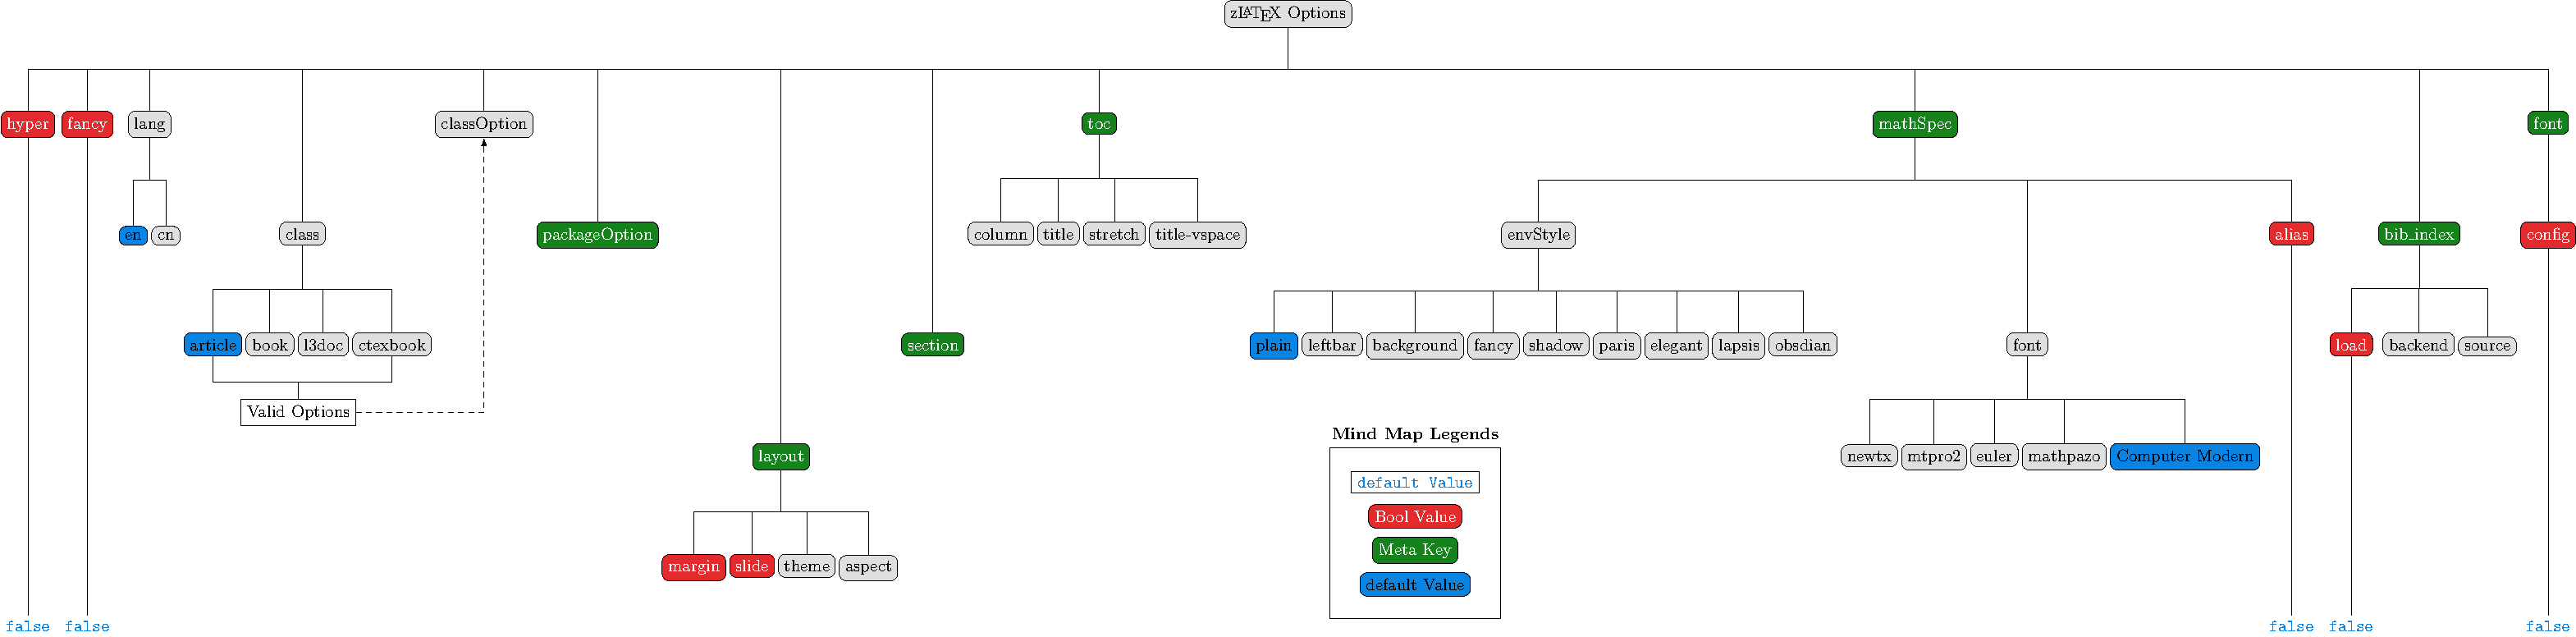
\includegraphics[width=1\linewidth]{zlatex_options.pdf}
  \caption{\zlatex{} 文档类选项示意图}
  \label{fig:zlatex-options}
\end{figure}

总体而言, \zlatex{} 的文档类选项是比较复杂的,对于刚接触本文档类的用户,不必知晓所有的选项配置,因为在默认的
选项配置下, \zlatex{} 已经能够得到一个效果较佳的文档了. 下面我们将详细介绍各个 \meta{key} 的指定方式及其具体含义.


\begin{function}[updated=2024-11-05]{\zlatexloadmodule, \zlatexloadlibrary}
  \begin{syntax}
    \cs{zlatexloadmodule}\marg{module name}
    \cs{zlatexloadlibrary}\marg{library name}
  \end{syntax}
  可以使用这两个命令用于加载 \zlatex 的模块和库,所有的 module 默认全部加载,library 默认全部不加载,
  由用户指定加载. 目前已有的 module 和 library 列表如下:

  \noindent\parbox[t]{.5\linewidth}{
    \noindent \textbf{module 列表:}
    \begin{itemize}
      \item \file{zlatex.module.fontcfg.tex}
      \item \file{zlatex.module.indexref.tex}
      \item \file{zlatex.module.layout.tex}
      \item \file{zlatex.module.pageinfo.tex}
      \item \file{zlatex.module.theme.tex}
      \item \file{zlatex.module.thm.tex}
      \item \file{zlatex.module.titlesec.tex}
      \item \file{zlatex.module.toc.tex}
    \end{itemize}}%
  \parbox[t]{.5\linewidth}{
    \noindent \textbf{library 列表:}
    \begin{itemize}
      \item \file{zlatex.library.fancy.tex}
      \item \file{zlatex.library.mathalias.tex}
      \item \file{zlatex.library.slide.tex}
      \item \file{zlatex.library.theme.tex}
    \end{itemize}}
\end{function}

各个 module 和 library 的加载方式请参见如下示例:
\begin{DocExample}
% \documentclass{zlatex}
\zlatexloadlibrary/\zarg{fancy}/
\zlatexloadlibrary/\zarg{mathalias}/
\zlatexloadlibrary/\zarg{slide}/
\zlatexloadlibrary/\zarg{theme}/
\end{DocExample}

你当然可以编写一个你自己的 module, 不妨假设其名称为 \meta{moduleA}; 将此文件命名为 \texttt{zlatex.module.\meta{moduleA}.tex}, 
然后将其放入路径 \meta{z\TeX}\file{/module/} 下,最后使用如下命令加载此 module:
\begin{DocExample}
\zlatexloadmodule{/\meta{moduleA}/}
\end{DocExample}

\begin{function}[rEXP, updated=2024-11-05]{lang}
  \begin{syntax}
    lang=\meta{cn, \zdefault*{en}}
  \end{syntax}
  \zlatex{} 目前仅对中英文做了适配,对于法语仅有部分支持. 根据不同的文档类语言,\zlatex{}会加载不同的和语言相关的
  宏包\index{language packages},不同\meta{lang}设置下, 宏包的加载情况为:
\end{function}
\begin{table}[!htb]
  \begin{tblr}{
    colspec={|X[1, c]|X[1.5, c]|X[1, c]|X[1, c]|X[1, c]|},
    rowspec={|Q[m]|Q[m]|}
  }
  lang=en & \pkg{inputenc}(\hologo{pdfTeX}) & \pkg{fontenc} & \pkg{babel} & \pkg{microtype} \\
  lang=cn & \pkg{fontspec} & \pkg{ctex} \\
  \end{tblr}
  \caption{\zlatex{} 文档类语言宏包}
  \label{tab:lang-package}
\end{table}

\begin{function}[rEXP, updated=2024-11-05]{hyper}
  \begin{syntax}
    hyper=\meta{true, \zdefault*{false}} 
  \end{syntax}
  是否开启文档内部的超链接以及 PDF 书签,默认为\zlatexVerb{false}. 建议在最后的成稿中启用此选项,在草稿
  阶段置为 \zlatexVerb{false} 可以加快文档的编译速度.
\end{function}

\begin{function}[rEXP, updated=2024-11-05]{fancy}
  \begin{syntax}
    fancy=\meta{true, \zdefault*{false}} 
  \end{syntax}
  此选项用于控制文档的外观,包括章节样式,定理类环境样式,默认为\zlatexVerb{false}. 
\end{function}

\begin{function}[rEXP, updated=2024-11-05]{class}
  \begin{syntax}
    class=\meta{\zdefault*{article}, book, ctexbook} 
  \end{syntax}
  此选项用于指定加载的基文档类,默认为 \cls{article}. 在加载 \cls{ctexbook}文档类后可以使用此文档类
  提供的 \cmd{\ctexset} 命令进行相关选项的配置. 
\end{function}

\begin{function}[rEXP, updated=2024-11-05]{classOption}
  \begin{syntax}
    classOption=\meta{class options} 
  \end{syntax}
  此选项接受一个逗号分隔的列表, 用于传递基文档类选项,针对默认的 \cls{article} 文档类,此项为\zlatexVerb{oneside, 12pt}. 一个简单的 
  设置样例:
\begin{DocExample}
\documentclass[
  class=article,
  classOption={10pt, leqno, a4paper},
]{zlatex}
\end{DocExample}
\end{function}

\begin{function}[rEXP, updated=2024-11-20]{packageOption}
  \begin{syntax}
    packageOption=\meta{key-value} 
  \end{syntax}
  此选项接受一个键值对, 用于给不同宏包传递选项, 使用样例:
\end{function}
\begin{DocExample}
\documentclass[
  packageOption={
    fontspec=quiet, 
    ctex={scheme=plain, punct=quanjiao},
  },
]{zlatex}
\end{DocExample} 

\begin{function}[updated=2024-12-25]{toc}
  \begin{syntax}
    toc=\meta{key-value}
  \end{syntax}
  此选项用于设置目录的样式,所有可选配置项如下:
\end{function}
\begin{DocExample}
\zlatexSetup{
  toc={
    column=/\meta{int\zdefault{1}}/,
    title=/\meta{tl\zdefault{Contents}}/,
    title-vspace=/\meta{dim\zdefault{-2em}}/,
    stretch=/\meta{float\zdefault{1}}/
  }
}
\end{DocExample}
若上述的 $\meta{column} \ge 2$, 那么 \zlatex{} 会自动加载\pkg{multicol}宏包. 注意: 由于在 \LaTeX{} 中,文档类选项不能含有控制序列,所以如果上述的 \meta{toc} 的某一个子项中含有控制序列,
那么务必通过命令 \cmd{\zlatexSetup} 进行设置, 示例如下:
\begin{DocExample}
\zlatexSetup{
  toc={
      title=\hfill\large\normalfont CONTENTS {\sffamily\small NEW}\hfill
    }
}
\end{DocExample}

\begin{function}[rEXP, updated=2024-12-06]{font}
  \begin{syntax}
    font = \meta{key-value}
  \end{syntax}
  此选项目前在实验性阶段,主要用于字体配置, 默认为\zlatexVerb{false}. 在启用此选项后,\zlatex{} 会自动加载
  \pkg{fontspec} 宏包,此时需更换引擎为\hologo{XeLaTeX} 或者 \hologo{LuaLaTeX}. 目前所有可选值如下:
\end{function}
\begin{DocExample}
\documentclass[
  font={config=/\meta{true, \zdefault*{false}}/}
]{zlatex}
\end{DocExample}


\begin{function}[rEXP, updated=2024-11-05]{layout}
  \begin{syntax}
    layout=\meta{key-value}
  \end{syntax}
  设置文档布局,所有可选配置项如下:
\end{function}
\begin{DocExample}
\documentclass[
  layout={
    margin=/\meta{bool\zdefault{false}}/,
    slide=/\meta{bool\zdefault{false}}/,
    aspect=/\meta{float|float\zdefault{12|9}}/,
    theme=/\meta{str\zdefault{AnnArborDefault}}/
  },
]{zlatex}
\end{DocExample}
在加载 \file{slide} library 后, 如果设置\meta{slide}\texttt{=true}, 那么此时即可把文档转为 slide 模式。

\begin{function}[updated=2024-12-05]{bib_index}
  \begin{syntax}
    bib_index=\meta{key-value}
  \end{syntax}
  此选项用于控制文档是否生成索引和参考文献,所有可用的选项为:
\end{function}
\begin{DocExample}
\zlatexSetup{
  bib_index={
    load=/\meta{bool\zdefault{false}}/,
    source=/\meta{str\zdefault{ref.bib}}/,
    backend=/\meta{str\zdefault{biber}}/
  }
}
\end{DocExample}
\meta{load} 用于控制是否加载 \pkg{biblatex} 宏包, 默认为 \zlatexVerb{false}; \meta{source} 用于指定参考文献源文件, 默认
文件名为:\file{ref.bib}; \meta{backend} 用于指定参考文献的后端,默认为 {biber}.


\begin{function}[updated=2024-11-05]{mathSpec}
  \begin{syntax}
    mathSpec=\meta{key-value}
  \end{syntax}
  此键用于配置数学排版相关选项. 所有可用的选项为:
\end{function}
\begin{DocExample}
\zlatexSetup{
  mathSpec={
    alias=/\meta{bool\zdefault{false}}/,
    envStyle=/\meta{tl\zdefault{plain}}/,
    font=/\meta{choice\zdefault{ncmrm}}/
  }
}
\end{DocExample}

\meta{alias} 默认为\zlatexVerb{false}, 当置为\zlatexVerb{true} 时,\zlatex{} 会加载\file{mathalias}库, 其中包含一系列
命令的简写声明, 如 \cmd{\ZZ} 代替 \zlatexVerb{\mathbb{Z}}; \meta{envStyle} 用于指定数学环境的样式, 默认为 \zlatexVerb{plain},
为了编译速度考虑,尽管 \zlatex{} 预定义了一系列的环境样式,但并不会预加载全部的样式, 而是把部分的样式移入了 \file{theme} 库中. 详细的
预定义样式列表如下:

\noindent\parbox[t]{.5\linewidth}{
\noindent \textbf{\pkg{thm} module 定义样式}:
\begin{itemize}
  \item plain 
  \item background
  \item leftbar 
  \item fancy 
\end{itemize}}%
\parbox[t]{.5\linewidth}{
\noindent \textbf{\pkg{theme} library 定义样式}:
\begin{itemize}
  \item shadow
  \item paris 
  \item elegant
  \item obsidian
  \item lapsis
\end{itemize}}

\meta{font} 用于指定数学公式字体,预定义的字体有:\zlatexVerb{newtx, euler, mtpro2, mathpazo}. 其中 \zlatexVerb{mtpro2}
为付费字体,需用户手动安装.


\clearpage
\section{杂项}
本小节会列举部分在 \cls{zlatex} 源文件中定义的命令, 这部分命令未迁移到任何的 module 或者是 library 中.

\begin{function}[updated=2024-11-05]{\zlatexVerb}
  \begin{syntax}
    \cs{zlatexVerb}\oarg{format}\marg{item}
  \end{syntax}
  此命令和 \hologo{LaTeX2e} 中的 \cmd{\verb} 类似,用于输出控制序列名称. 和后者类似,此命令也不能作为
  任何控制序列的参数. \meta{format} 用于指定控制序列的打印格式, 默认为 \zlatexVerb{\texttt}. 一个使用
  样例如下:
\end{function}
\begin{DocExample}*
  \zlatexVerb{\alpha + \beta}\par
  \zlatexVerb[\textsf]{\alpha + \beta}
\end{DocExample}


\begin{function}[added=2024-11-05]{\graphicspath}
  \begin{syntax}
    \cs{graphicspath}\marg{path}
  \end{syntax}
  此命令用于指定图片的搜索路径, 此命令来自 \pkg{graphicx} 宏包, 默认设置为:
\end{function}
\begin{DocExample}
  \graphicspath{
    {./figure/}{./figures/}{./image/}{./images/}
    {./Pictures/}{./picture/}{./Pics/}{./pics/}
    {./graphics/}{./graphic/}
  }
\end{DocExample}


\begin{function}[updated=2024-11-05]{\zlatexCounterWith}
  \begin{syntax}
    \cs{zlatexCounterWith}\marg{child}\marg{parent}
  \end{syntax}
  此命令用于给一个计数器添加一个父计数器, 当 \meta{parent} 计数器增加时,\meta{child} 计数器会自动重置.
  本命令为 \cmd{\@addtoreset} 的封装.
\end{function}


\begin{function}[added=2025-02-04]{\counterwithin}
  \begin{syntax}
    \cs{counterwithin}\marg{child}\marg{parent}
  \end{syntax}
  此命令用于给一个计数器 \meta{child} 设置一个父计数器, 当 \meta{parent} 计数器增加时,\meta{child} 计数器会自动重置.
  本命令和命令 \cmd{\@addtoreset} 的作用类似.
\end{function}


\begin{function}[updated=2024-11-05]{\zlatexFramed}
  \begin{syntax}
    \cs{zlatexFramed}\oarg{color}\marg{name}
  \end{syntax}
  此命令用于创建一个类似 MarkDown 中引用环境, \meta{color} 表示环境 \meta{name} 的默认颜色,在使用环境
  \meta{name} 时可以更改 \meta{color} 这一默认的可选参数. 一个使用样例如下:
\end{function}
\begin{DocExample}*
  \zlatexFramed[red]{ref}
  \begin{ref}This is a simple ref env.\end{ref}
  \begin{ref}[green]This is a simple ref env.\end{ref}
\end{DocExample}


\begin{function}[updated=2024-12-05]{\c_zlatex_quad_dim}
  \begin{syntax}
    \cs{c_zlatex_quad_dim}
  \end{syntax}
  此命令表示当前文档中一个空格的宽度.
\end{function}


\begin{function}[added=2025-01-17]{zlatex-title-page, zlatex-last-page}
  \begin{syntax}
    \cmd{\pageref}\zarg{zlatex-title-page}
    \cmd{\pageref}\zarg{zlatex-last-page}
  \end{syntax}
  引用当前文档的最后一页, 可以在制作页眉页脚格式时使用. 但对应的超链接跳转也许并不正确, 此时
  应使用 \texttt{zlatex@lastpage} 这一 anchor. 一个基本的使用样例如下:
\end{function}
\begin{DocExample}*
  \pageref{zlatex-title-page}--\pageref{zlatex-last-page}
\end{DocExample}


\begin{function}[added=2025-01-17]{zlatex@titlepage, zlatex@lastpage}
  \begin{syntax}
    \cs{hyper@link}\marg{context}\zarg{zlatex@titlepage}\marg{link text}
    \cs{hyper@link}\marg{context}\zarg{zlatex@lastpage}\marg{link text}
  \end{syntax}
  上述两 Targets 由命令 \cs{hyper@anchor} 设置, 分别应用于引用当前文档的第一页和最后一页, 在 \zlatex{} 中, 标题页的页码为 1.

  注意:普通用户不应该直接使用这两个 Targets,此二 Targets 主要提供给模板的开发者, 用户应使用位于首页和尾页的 \texttt{zlatex-title-page} 
  和 \texttt{zlatex-last-page} 两 label.
\end{function}


\begin{function}[updated=2024-11-05]{\zlatexTitle, \zlatexAuthor, \zlatexDate}
  \begin{syntax}
    \cs{zlatexTitle}
    \cs{zlatexAuthor}
    \cs{zlatexDate}
  \end{syntax}
  此三个命令用于分别保存导言区 \cmd{\@title}, \cmd{\@author}, \cmd{\@date} 三个变量的值, 
  用户可以在正文部分使用此三个变量. 一个使用样例如下:
\end{function}
\begin{DocExample}*
  \zlatexTitle\par
  \zlatexAuthor\par
  \zlatexDate
\end{DocExample}


\clearpage
\section{状态检测}
因 \zlatex{} 的选项配置比较庞大,其中涉及到诸多的宏包和命令的加载,所以在文档编译时,我们需要对文档的各种状态进行检测,
\zlatex{} 提供了一系列的命令用于检测文档中各个变量状态的命令.

\begin{function}[added=2025-01-15, EXP]{\zlatexHyperTF, \zlatexFancyTF, \zlatexMarginTF, \zlatexSlideTF, \zlatexFontConfigTF, \zlatexMathAliasTF, \zlatexBibIndexLoadTF, \zlatexThemeLibLoadTF}
  \begin{syntax}
    \cs{zlatexHyperTF}\marg{true code}\marg{false code}
  \end{syntax}
  此命令用于检测当前文档中是否开启了超链接功能,如果开启了,那么执行 \meta{true code}, 否则执行 \meta{false code}, 其余命令的使用方法同理. 各个检测命令的基本使用样例如下:
\end{function}
\begin{DocExample}*
\zlatexHyperTF{Hyperref is loaded.}{Hyperref is not loaded.}\par
\zlatexFancyTF{Fancy is loaded.}{Fancy is not loaded.}\par
\zlatexMarginTF{Margin does set.}{Margin does NOT set.}\par
\zlatexSlideTF{Slide is loaded.}{Slide is not loaded.}\par
\zlatexFontConfigTF{Font config is loaded.}{Font config is not loaded.}\par
\zlatexMathAliasTF{Math alias is loaded.}{Math alias is not loaded.}\par
\zlatexBibIndexLoadTF{Bib index is loaded.}{Bib index is not loaded.}\par  
\zlatexThemeLibLoadTF{Theme library is loaded.}{Theme library is not loaded.}
\end{DocExample}


\clearpage
\section{Modules}
本节对应的所有 module 默认自动加载,用户仍可以通过命令 \cmd{\zlatexloadmodule} 调用自己编写的 module.

\subsection{fontcfg}
本模块主要用于配置 \zlatex{} 的字体, 尽管 \pkg{fontspec} 和 \pkg{unicode-math} 已经在很大程度上
简化了字体的配置,但是对于一些用户来说,仍然会感到困扰. 本模块的目的就是为了简化字体的配置,让普通的
\LaTeX{} 用户也能够方便的配置字体, 用上自己喜欢的字体. 

\begin{function}[updated=2024-12-05]{\Cinzel}
  \begin{syntax}
    \cmd{\Cinzel}
  \end{syntax}
  本命令用于临时切换 Cinzel 字体(此时需使用 \hologo{XeLaTeX} 或 \hologo{LuaLaTeX}), 本字体在 \meta{fancy}\zlatexVerb{=true} 时,会自动应用于 chapter 页的字体.
\end{function}

\begin{function}[updated=2024-12-05]{\blacktriangleright}
\begin{syntax}
  \cs{blacktriangleright}
\end{syntax}
本命令(符号)来自 AMSa 字体, \meta{slot}\zlatexVerb{="49}. 主要用于在 \meta{slide}\zlatexVerb{=true} 时对此符号进行 Patch.
\end{function}


\clearpage
\subsection{indexref}
本模块主要用于给文档增加索引,参考文献以及超链接支持, 通过本模块,用户可以方便的添加索引, 参考文献以及超链接.

% \makeatletter
\begin{function}[added=2024-12-05]{\hyper@anchor}
  \begin{syntax}
    \cs{hyper@anchor}\marg{destination name}
  \end{syntax}
  此命令用于创建一个超链接锚点, \meta{destination name} 作为后续超链接命令的跳转目标.
\end{function}


\begin{function}[added=2024-12-05]{\hyper@link}
  \begin{syntax}
    \cmd{\hyper@link}\marg{context}\marg{destination name}\marg{link text}
  \end{syntax}
  此命令用于创建一个超链接, \meta{link text} 本身作为一个超链接对象,点击\meta{link text} 即可跳转到对
  应的 \meta{destination name}. \meta{context} 表示此链接所属的类型, 默认有: \texttt{link, url, cite} 三种类型.
\end{function}

\begin{function}[added=2024-12-05]{\hyper@linkstart}
  \begin{syntax}
    \cmd{\hyper@linkstart}\marg{context}\marg{destination name}
  \end{syntax}
  此命令用于开启一个超链接\textbf{域}, 此\textbf{域}中的内容可以是任意的文本或其它图片对象. 此命令需结合后续的
  \cmd{\hyper@linkend} 命令使用,此二命令结合使用时基本和上述的 \cmd{\hyper@link} 命令基本等效.
\end{function}


\begin{function}[added=2024-12-05]{\hyper@linkend}
  \begin{syntax}
    \cmd{\hyper@linkend}
  \end{syntax}
  用于结束由 \cmd{\hyper@linkstart} 开启的\textbf{域}.
\end{function}


\begin{function}[added=2024-12-05]{\hyper@linkfile}
  \begin{syntax}
    \cmd{\hyper@linkfile}\marg{link text}\marg{filename}\marg{destname}
  \end{syntax}
  此命令用于创建一个超链接, 点击\meta{link text} 即可跳转到对应的 \meta{filename} 文件中的 \meta{destname} 处.
\end{function}

\begin{function}[added=2024-12-05]{\MakeLinkTarget,\MakeLinkTarget*}
  \begin{syntax}
  \cs{MakeLinkTarget}\oarg{prefix}\marg{counter}
  \cs{MakeLinkTarget}*\marg{target}
  \end{syntax}
  此二命令用于在用户层面创建超链接跳转目标,其中 \meta{prefix} 和 \meta{counter} 可以作为命令
  \cmd{\hyper@link} 的参数使用. \meta{counter} 可以为 \texttt{chapter, section, subsection} 等.
  针对 \cs{MakeLinkTarget*}, 其中 \meta{target} 可以为任意的 Unicode 文本(但为了兼容性考虑,请尽量使用 ASCII 字符).
\end{function}


\begin{function}[added=2024-12-05]{\LinkTargetOn, \LinkTargetOff}
  \begin{syntax}
    \cs{LinkTargetOn}
    \cs{LinkTargetOff}
  \end{syntax}
  此命令常在一个局部中用于取消由 \cs{MakeLinkTarget} 或 \cs{refstepcounter} 创建的 Target. 在使用 
  \cs{LinkTargetOff} 后,你仍然可以在一个局部里重新启用超链接然后创建对应的 Target, 示例如下:
\end{function}
\begin{DocExample}
\LinkTargetOff  % suppress anchor in internal refstepcounter
...
\refstepcounter{...}
...
{\LinkTargetOn\MakeLinkTarget*{mytarget}} % create manual anchor for future reference
...
\LinkTargetOn
\end{DocExample}


\begin{function}[added=2024-12-05]{\NextLinkTarget}
  \begin{syntax}
    \cs{NextLinkTarget}\marg{target}
  \end{syntax}
  此命令设置下一个由 \cs{MakeLinkTarget} 或 \cs{refstepcounter} 创建的 target. 此命令的作用和 
  \cs{hypersetup} 中的 \cmd{next-anchor} 类似.
\end{function}
% \makeatother


\begin{function}[added=2024-12-05]{\SetLinkTargetFilter}
  \begin{syntax}
    \cs{SetLinkTargetFilter}\marg{filter}
  \end{syntax}
  此命令用于给当前文档中所有的 Link Target 添加一个前缀,此命令在合并多个不同的 PDF 时是十分有用的. 
\end{function}

\begin{function}[added=2025-04-21]{\cref}
  \begin{syntax}
    \cs{cref}\marg{labels}
    \cs{cref}\oarg{options}\marg{labels}
  \end{syntax}
  \zLaTeX{} 基于 \pkg{cleveref} 和 \pkg{zref-clever} 宏包提供 ``聪明引用'' 命令 \cs{cref}. (\textcolor{red}{\sffamily 目前% 
  \pkg{cleveref} 宏包的维护情况不太明朗, 且和新版的 \TeX{}Live 中的部分宏集冲突, 这便是 \zLaTeX{} 同时提供二者的原因}). 为统一命令, 
  \zLaTeX{} (仅)将 \pkg{zref-clever} 中的 \cmd{\zcref} 重定义为 \cmd{\cref}, 方便用户的使用. \textbf{注意:} 尽管二者名称相同但各命令的
  需要的参数格式是不同的,其余命令同理, 详情请参考对应的手册. 用户可以通过本文档类的 \meta{cref-backend} 选项进行后端的设置, 默认后端为 
  \pkg{zref-clever} 一个简单的设置样例如下:
\end{function}
\begin{DocExample}
\documentclass[cref-backend=zref-clever]{zlatex}
\end{DocExample}


\clearpage
\subsection{layout}
本模块主要用于设置文章布局,包括纸张大小,页边距等.

\begin{function}[added=2025-04-21]{\geometry}
  \begin{syntax}
    \cmd{\geometry}\marg{key-value}
  \end{syntax}
  此命令来自 \pkg{geometry} 宏包, 用户可以直接在导言区使用, 详细的使用方法请参见 \pkg{geometry} 宏包 
  文档.
\end{function}

\begin{function}[added=2025-04-21]{\setuplayout}
  \begin{syntax}
    \cs{setuplayout}\marg{layout key-val}
    \cs{setuplayout}\oarg{preset name}\marg{layout key-val}
    \cs{setuplayout}*\oarg{preset name}\marg{layout key-val}
  \end{syntax}
  此命令由 \CusTeX{} 宏集提供, 详细的使用方法请参见其手册.
\end{function}


\clearpage
\subsection{pageinfo}
本模块主要包含与页面生成以及页面标注相关(页眉页脚)的命令, 如 \cmd{\maketitle},\-\cmd{\zlatexPageMask}; 
通过本模块,用户可以方便制作独特的页面样式以及水印添加.

\begin{function}[updated=2024-11-05]{\orimaketitle}
  \begin{syntax}
    \cs{orimaketitle}
  \end{syntax}
  \cs{maketitle} 的原始形式.
\end{function}

\begin{function}[updated=2024-11-05]{\maketitle}
  \begin{syntax}
    \cs{maketitle}
  \end{syntax}
  \zlatex{} 对原始的 \cs{maketitle} 进行了重定义,以适应不同的文档类和页面布局.
\end{function}

\begin{function}[added=2024-12-05]{\Maketitle}
  \begin{syntax}
    \cs{Maketitle}\oarg{margin\zdefault{1in}}
  \end{syntax}
  此命令会忽略所有的文档类选项或者是页面布局,在新的页面布局中插入 \cmd{\maketitle} 的原始定义, \meta{margin} 
  表示新的页面布局的 margin, 默认为 \texttt{1in}. 此命令的实现为:
\end{function}
\begin{DocExample}
\newcommand\Maketitle[1][1in]{
  \newgeometry{margin=#1}
  \orimaketitle
  \restoregeometry
}
\end{DocExample}


\begin{function}[updated=2024-11-05]{\frontmatter, \mainmatter}
  \begin{syntax}
    \cs{frontmatter}
    \cs{mainmatter}
  \end{syntax}
  此二命令用于设置文档的前言和正文部分,在 \zlatex{} 中这两个命令已经被重定义,当加载的 \meta{class} 为 \cls{book} 或 \cls{ctexbook} 时,
  这两个命令会自动处理页眉页脚相关设置.
\end{function}

\begin{function}[updated=2024-12-05]{\__zlatex_page_annotate:nnnnn}
  \begin{syntax}
    \cmd{\__zlatex_page_annotate:nnnnn} \marg{fore/background}
      \marg{position}\marg{anchor}
      \marg{object}\marg{hook range}
  \end{syntax}
  此命令为 \cmd{\zlatexPageMask} 的底层命令, 用户可以依据此命令创建更加具有针对性的水印命令.
\end{function}

\begin{function}[updated=2024-12-05]{\zlatexPageMask, \zlatexPageMask*}
  \begin{syntax}
    \cs{zlatexPageMask}\oarg{key-value}\marg{item}
  \end{syntax}
  命令 \cmd{\zlatexPageMask} 用于给当前页面添加水印,\cmd{\zlatexPageMask*} 用于给当前页面及其之后的所有
  页面添加水印. \meta{item} 可以为一段文字,也可以为一系列的图片(需要使用\cmd\includegraphics 进行导入). 
  \meta{key-value} 所有可用的选项为:
\end{function}
\begin{DocExample}
  \zlatexPageMask[
    layer=/\meta{tl:\zdefault*{background}, foreground}/, 
    position=/\meta{tl:(dim1, dim2)}/,
    label=/\meta{tl:\zdefault*{DEFAULT}}/, 
    anchor=/\meta{tl:\zdefault*{c}, tl, tc, tr, bl, bc, br, etc}/
  ]{/\meta{item}/}
\end{DocExample}
其中\meta{position}以页面的左下角为原点,向上向右为正方向. \meta{anchor} 为两个字符: 一个为水平位置,另一个为垂直位置。
水平位置包括:左(\texttt{l})、中(\texttt{c})、右(\texttt{r})、内侧(\texttt{i})、外侧(\texttt{o});垂直位置包括:
顶部(\texttt{t})、中部(\texttt{m})、底部(\texttt{b}). 

注意: \pkg{transparent}宏包仅可以在 \hologo{pdfLaTeX} 和 \hologo{LuaLaTeX} 下正常工作. 一个简单的示例, 给当前页面添加一个水印:
\begin{DocExample}*
  % \usepackage{tikzlings}
  \zlatexPageMask{
    \transparent{.5}
\includegraphics{latex-logo.pdf}
  }
  \zlatexPageMask[anchor=tr, position={(\zpw, \zph)}]{
    \begin{tikzpicture}[scale=2]
      \marmot
    \end{tikzpicture}
  }
\end{DocExample}
上述的 \cmd{\zpw}, \cmd{\zph} 分别表示当前纸张的宽和高.


\begin{function}[added=2024-12-05]{\zpw, \zph}
  \begin{syntax}
    \cs{zpw}
    \cs{zph}
  \end{syntax}
  此二命令表示当前纸张的宽和高, 命令原型为 \cs{paperwidth} 和 \cs{paperheight}.
\end{function}

\begin{function}[added=2024-12-05]{\zlatexPageMaskRemove}
  \begin{syntax}
    \cs{zlatexPageMaskRemove}\marg{foreground/backgroud}\marg{label}
  \end{syntax}
  此命令用于移除由 \cmd{\zlatexPageMask} 命令添加的页面水印, \meta{label} 即为 \cmd{\zlatexPageMask} 可选
  参数 \meta{key-value} 中 \meta{label} 对应的 value. 如果 \meta{label} 对应的水印并不存在, \zlatex{} 会抛出警告.
\end{function}

\vskip3em
\noindent\textcolor{red}{\sffamily 目前可以使用 \CusTeX{} 提供的接口进行定制, 请参见其 \pkg{bgfg} 模块.}


\clearpage
\subsection{theme}
本模块主要用于文档装饰,在本模块中定义了一系列的颜色主题,这系列主题可以应用于文章中的各个元素,包括但不限于
章节标题, 定理环境, 超链接跳转,(子)目录样式.

\begin{function}[updated=2024-11-05]{\zlatexColorSetup}
  \begin{syntax}
    \cs{zlatexColorSetup}\marg{key-value}
  \end{syntax}
  当 \meta{hype}\zlatexVerb{=true} 时, 此命令可以用于设置文档中各种元素的色彩, 但仅可在导言区使用. \zlatex{} 把文档
  中的元素分为如下的 3 类:
  \begin{itemize}
    \item 章节标题类: \zlatexVerb{chapter, chapter-rule};
    \item 超链接类: \zlatexVerb{link, cite, url};
    \item 数学环境类: \env{axiom, definition, theorem, lemma, corollary, proposition, remark, proof, exercise, example, solution, problem}.
  \end{itemize}
  在颜色指定上,\zlatex{} 实现了一套自己的颜色指定方式, 在指定色彩时可以不必要提前定义. 参见如下使用案例:
  \begin{DocExample}
    \zlatexColorSetup{
      chapter = red,
      link = {HTML}{d9d9d9},
      theorem = {RGB}{136, 63, 214}
    }
  \end{DocExample}
\end{function}

\zlatex{} 部分默认配色\Footnote{zchapColor 还未整理, 目前只能单独重定义}如下:
\begin{table}[H]
  \begin{tblr}{
    colspec={|X[1.25, c]|X[1.1, c]|X[1.85, c]|X[1.2, c]|X[.9, c]|X[1.65, c]|X[2, c]|X[1.75, c]|},
    rowspec={|Q[m]|Q[m]|Q[m]|Q[m]|},
    cells={cmd=\small\env}
  }
    Struct & chapter & chap-rule & link & url & cite  & chap-theme  & slide-theme\\ 
    Color & \block{RoyalRed} & \block{black} & \block{purple}& \block{RoyalRed} & \block{blue} & \block{zchapColor} & \block{Ann-default-I}\\
    MathEnv & axiom & definition & theorem & lemma & corollary & proposition & remark \\  
    Color & \block{zlatex@color@axiom} & \block{zlatex@color@definition} & \block{zlatex@color@theorem} & 
    \block{zlatex@color@lemma}& \block{zlatex@color@corollary}& \block{zlatex@color@proposition}& \block{zlatex@color@remark}\\
  \end{tblr}
  \caption{z\LaTeX{}文档类默认配色}
  \label{tab:zlatex-default-color}
\end{table}

定理类环境的色彩保存于变量 \cmd{zlatex@color@\meta{name}} 中, 其中 \meta{name} 为对应环境的名称. 不推荐用户 使用命令 \cmd{\definecolor}, \cmd{\colorlet} 
直接对这类色彩变量进行重定义, \zlatex{} 鼓励用户通过 \cmd{\zlatexColorSetup} 命令进行色彩的重定义.

注意: \cmd{\zlatexThmColorSetup} 仅能用于数学类环境的色彩自定义, 所以对于 \texttt{link, chapter} 等色彩请使用 \cmd{\zlatexColorSetup} 命令进行设置.

\begin{function}[updated=2024-12-05]{\__zlatex_color_set:n}
  \begin{syntax}
    \cmd{\__zlatex_color_set:n} \marg{color spec}
  \end{syntax}
  此命令可以自动解析 \meta{color spec}, 并以此创建或定义对应的色彩. \meta{color spec} 可以为普通的
  预定义色彩名,如 \texttt{red, orange} 等. 亦或者是 \texttt{HTML, RGB, CMYK} 等色彩模型,但此时的格式略有
  不同。此命令仅能在 \cmd{\keys_define:nn} 中使用,新定义的色彩名为 \zlatexVerb{zlatex@color@\l_keys_key_str}. 
  关于参数 \meta{color spec} 的使用,可以参见如下示例:
\end{function}
\begin{DocExample}*
  \ExplSyntaxOn
  \keys_define:nn {colorTest}{
    keyA    .tl_set:N     =  \l__zlatex_keyA_color_tl,
    keyA    .code:n       =  { \__zlatex_color_set:n {#1} },
  }
  \keys_set:nn {colorTest}{keyA={HTML}{d9d9d9}}
  \textcolor{zlatex@color@keyA}{This~is~a~test.}
  \ExplSyntaxOff
\end{DocExample}


\clearpage
\subsection{thm}
本模块主要用于定理类以及证明类数学环境定制. 本模块提供了丰富的接口以及选项,与此同时本模块提供了丰富的
Hook, 方便用户直接对环境进行操作.

\pkg{thm} 提供的数学环境主要分为两类:
\begin{itemize}
  \item 定理类: \env{axiom, definition, theorem, lemma, corollary, proposition, remark};
  \item 证明类: \env{proof, exercise, example, solution, problem}
\end{itemize}

所以请区分 ``定理类'' 和 ``证明类'' 两类环境, 以便于正确地使用 \pkg{thm} 提供的各个命令. \zlatex{} 的 \pkg{thm} module 
中的部分命令或变量也许没有显式地含有 \textcolor{red}{theorem} 字样, 但是这些命令或变量仍然是属于 ``定理类'' 的; 应用于
``证明类'' 环境的命令或变量均显式地含有 \textcolor{red}{proof} 字样.


\begin{function}[updated=2024-11-05]{\zlatexThmLang}
  \begin{syntax}
    \cs{zlatexThmLang}\marg{lang}
  \end{syntax}
  此命令用于设置定理类环境的名称, 目前支持 \texttt{cn, en, fr} 三种语言. 此命令仅能在文档的导言区使用, 但为了说明此命
  令的使用方法,在本手册中,此命令的定义被临时改变了. 一个使用样例如下:
\end{function}
\begingroup
\begin{DocExample}*
  \begin{theorem}[zlatexThmLang-1]
    This is a chinese zlatexThmLang-1.
  \end{theorem}
  \zlatexThmLang{fr}
  \begin{theorem}[zlatexThmLang-2]
    This is a france zlatexThmLang-2.
  \end{theorem}
  \zlatexThmLang{en}
  \begin{theorem}[zlatexThmLang-3]
    This is a english zlatexThmLang-3.
  \end{theorem}
\end{DocExample}
\endgroup


\begin{function}[added=2025-02-04]{\zlatexThmNameSet}
  \begin{syntax}
    \cs{zlatexThmNameSet}\marg{lang}\marg{key-value}
  \end{syntax}
  此命令用于设置数学环境的名称, 包括 ``定理类'' 和 ``证明类''. 此命令仅能在文档的导言区使用, 但为了说明此命
  令的使用方法,在本手册中,此命令的定义被临时改变了. 预定义的 \meta{lang} 值有: \texttt{en, cn, fr}, 用户 
  可以使用此命令自行配置, 然后使用命令 \cs{zlatexThmLang}\texttt{\{\meta{lang}\}} 进行切换. \meta{key-value} 的所有可用键
  即为所有的预定义数学环境名称. 一个使用样例如下:
\end{function}
\begin{DocExample}*
  \zlatexThmNameSet{cn}{
    theorem=新定理,
    proof=证
  }
  \zlatexThmLang{cn}
  \begin{theorem}[zlatexThmNameSet-1]
    This is a theorem zlatexThmNameSet-1.
  \end{theorem}
  \begin{proof}
    This is a proof.
  \end{proof}
\end{DocExample}

注意: 此命令需应用于 \cmd{\zlatexThmLang} 命令之前, 否则此命令的相关设置将不会生效.


\zlatexThmStyle{background}
\begin{function}[updated=2025-02-04]{\zlatexThmCreate}
  \begin{syntax}
    \cs{zlatexThmCreate}\oarg{type\zdefault{theorem}}\marg{spec}
  \end{syntax}
  根据 \meta{spec} 创建一系列类型为 \meta{type} 的定理环境, 如果对应的环境已存在,则覆盖其原有的定义. 
  \meta{type} 可选\zlatexVerb{theorem, proof}两种类型. 命令 \cmd{\zlatexThmCreate} 仅可在导言区使用, 但为了说明其使用方法,
  在本手册中,此命令的定义被临时改变了. 和前面的 \cmd{\zlatexColorSetup} 命令类似, 在指定色彩时可以不必要提前定义.
  % 注意: \meta{spec} 中类似 \cmd{Zsolution=Solution|} 这样的定义是不合法的, 此定义最后的 \cmd{|} 应被移除. 
  针对 \meta{spec}, 请参见下面的使用样例:
\end{function}
\begin{DocExample}*
  \zlatexThmCreate{Zaxiom, Ztheorem=Thm|{HTML}{a0d911}, Zproposition=Prop|blue}
  \zlatexThmCreate[proof]{Zproof, Zexample=EXAMPLE|red, Zsolution=Solution|}
  \begin{Zproof}[zlatexThmCreate-1]
    This is a Zproof zlatexThmCreate-1.
  \end{Zproof}
  \begin{Zexample}[zlatexThmCreate-2]
    This is a Zexample zlatexThmCreate-2.
  \end{Zexample}
  \begin{Ztheorem}[zlatexThmCreate-3]
    This is a Ztheorem zlatexThmCreate-3
  \end{Ztheorem}
\end{DocExample} 
\zlatexThmStyle{plain}

\begin{function}[EXP, updated=2024-11-05]{\zlatexThmNumber}
  \begin{syntax}
    \cs{zlatexThmNumber}
  \end{syntax}
  此命令表示对应环境的编号, 类似于 \pkg{amsthm} 中的 \cmd{\thmnumber}. 用户不应在除 \cmd{\zlatexThmTitleFormat} 外的
  任何地方使用, 在命令 \cs{zlatexThmTitleFormat} 之外, 此命令输出的内容无任何实际意义.
\end{function}

\begin{function}[EXP, updated=2024-11-05]{\zlatexThmName}
  \begin{syntax}
    \cs{zlatexThmName}
  \end{syntax}
  此命令表示对应环境的名称, 类似于 \pkg{amsthm} 中的 \cmd{\thmname}. 用户不应在除 \cmd{\zlatexThmTitleFormat} 外的
  任何地方使用, 在命令 \cs{zlatexThmTitleFormat} 之外, 此命令输出的内容无任何实际意义.
\end{function}

\begin{function}[EXP, updated=2024-12-05]{\zlatexThmNote}
  \begin{syntax}
    \cs{zlatexThmNote}\marg{prefix}\marg{suffix}
  \end{syntax}
  此命令表示对应环境的注释, 类似于 \pkg{amsthm} 中的 \cmd{\thmnote}. 用户不应在除 \cmd{\zlatexThmTitleFormat} 外的
  任何地方使用, 在命令 \cs{zlatexThmTitleFormat} 之外, 此命令输出的内容无任何实际意义.
\end{function}


\begin{function}[added=2025-04-22]{\thm@temp@name}
  \begin{syntax}
    \cs{thm@temp@name}
  \end{syntax}
  此命令用于临时保存定理类环境的名称, 用户可以在自定义定理类环境样式时使用. \textbf{注意}: 此命令和前述的
  \cmd{\zlatexThmName} 不同, 因 \cs{thm@temp@name} 只能取值于合法的定理类环境名称集合, 而 \cmd{\zlatexThmName}
  是 \cs{thm@temp@name} 的格式化版本, 可能包含 \cs{bfseries}, \cs{sffamily} 等格式化命令.
\end{function}


\begin{function}[added=2025-02-04]{\thm@temp@color, \thm@proof@temp@color}
  \begin{syntax}
    \cs{thm@temp@color}
    \cs{thm@proof@temp@color}
  \end{syntax}
  此二命令用于临时保存定理类环境和证明类环境的色彩, 用于在 \cmd{\zlatexThmTitleFormat} 中进行色彩切换.
  注意: 普通用户在使用这两个命令时, 请将其置于 \cs{makeatletter} 和 \cs{makeatother} 之间.
\end{function}


\begin{function}[EXP, updated=2024-11-05]{\zlatexThmTitle, \zlatexThmTitle*}
  \begin{syntax}
    \cs{zlatexThmTitle}
    \cs{zlatexThmTitle*}
  \end{syntax}
  \cs{zlatexThmTitle} 命令为定理类环境纯文本标题, 包含 \cmd{\zlatexThmNumber}, \cmd{\zlatexThmName}, \cmd{\zlatexThmNote} 三
  部分以及一些其它文本. \cs{zlatexThmTitle*} 为 \cs{zlatexThmTitle} 的格式化版本(可能包含 \cs{bfseries}, \cs{sffamily} 等格式化命令); 
  用户在自定义定理类环境样式时应优先使用 \cs{zlatexThmTitle*}, 此命令生成的定理类环境标题才能被 \cs{zlatexThmTitleFormat} 控制. 
  此二命令中文本的具体格式可以使用 \cmd{\zlatexThmTitleFormat} 进行指定.
\end{function}
% \clearpage


\begin{function}[updated=2024-11-05]{\zlatexThmTitleSwitch, \zlatexThmTitleSwitch*}
  \begin{syntax}
    \cs{zlatexThmTitleSwitch}
  \end{syntax}
  命令 \cmd{\zlatexThmTitleSwitch} 用于隐藏定理类环境的标题, 命令 \cmd{\zlatexThmTitleSwitch*} 用于显示标题; 在自定义环境
  样式时比较有用. 用户不应该对此命令进行直接的调用.
\end{function}
\begin{DocExample}*
  \begin{theorem}[zlatexThmTitleSwitch-1]
    A theorem zlatexThmTitleSwitch-1.
  \end{theorem}
  \zlatexThmStyleNew{
    ZZZ={begin=, end=, option=\zlatexThmTitleSwitch},
  }
  \zlatexThmStyle{ZZZ}
  \begin{theorem}[zlatexThmTitleSwitch-2]
    A theorem zlatexThmTitleSwitch-2.
  \end{theorem}
\end{DocExample}
关于命令 \cmd{\zlatexThmStyle} 的使用可以参见下面的说明.


\zlatexThmStyle{plain}
\begin{function}[updated=2025-02-04]{\zlatexThmTitleFormat, \zlatexThmTitleFormat*}
  \begin{syntax}
    \cs{zlatexThmTitleFormat}\oarg{type\zdefault{theorem}}\marg{format}
  \end{syntax}
  此命令用于修改类型为 \meta{type} 的数学类环境的标题格式, 即命令 \cmd{\zlatexThmTitle} 的内容, 仅能在导言区使用.% 
  \meta{type} 的可选值有: \texttt{theorem, proof}, 默认值为 \texttt{theorem}. 命令 \cs{zlatexThmTitleFormat} 仅应用于之后的第一个
  (类型为 \meta{type} 的)数学类环境标题样式, 而 \cs{zlatexThmTitleFormat*} 则应用于之后的所有(类型为 \meta{type} 的)数学类环境. 
  \meta{format} 的默认格式为(未考虑 \cs{zlatexThmNote} 为空的情况下):
\end{function}
\begin{DocExample}
  \zlatexThmName\ \zlatexThmNumber\ \zlatexThmNote{(}{)}
\end{DocExample}

此命令的一个简单使用案例如下:
\ExplSyntaxOn
\tl_set:Nn \l__zlatex_proof_color_tl {blue!50}
\ExplSyntaxOff
\begin{DocExample}*
\zlatexThmColorSetup{proof=blue!50}
\makeatletter
\zlatexThmTitleFormat{\bfseries\color{\thm@temp@color}\zlatexThmName\zlatexThmNote{\{}{\}}\zlatexThmNumber\ }
\zlatexThmTitleFormat[proof]{\color{\thm@proof@temp@color}\bfseries[:\zlatexThmName:]\ }
\makeatother
\begin{theorem}[zlatexThmTitleFormat-1]
  A theorem zlatexThmTitleFormat-1.
\end{theorem}
\begin{proof}
  This is a proof.
\end{proof}
\end{DocExample}
\ExplSyntaxOn
\tl_set:Nn \l__zlatex_proof_color_tl {black}
\ExplSyntaxOff

此外, 还可以参见命令 \cs{zlatexThmNoteEmptyTF} 中的使用示例. 

注意: 如果 \meta{type} 为 \texttt{proof}, 那么在 \meta{format} 中仅有 \cs{zlatexThmName} 和 \cs{thm@proof@temp@color} 可用.


\begin{function}[updated=2024-12-05]{\zlatexThmNoteEmptyTF}
  \begin{syntax}
    \cs{zlatexThmNoteEmptyTF}\marg{true code}\marg{false code}
  \end{syntax}
  此命令用于判断 \cmd{\zlatexThmNote} 是否为空, 如果为空则执行 \meta{true code}, 否则执行 \meta{false code}.
  这个命令在自定义 \cmd{\zlatexThmTitle} 时很有用. 一个使用样例(\zlatex{} 内置的 \zlatexVerb{obsidian} 定理样式对应
  的格式, 具体效果可以参见: \cref{sec:theme-library-obsidian}):
\end{function}
\begin{DocExample}
\zlatexThmTitleFormat*{\bfseries
  \zlatexThmName\ \zlatexThmNumber
  \zlatexThmNoteEmptyTF{}{\\}
  \zlatexThmNote{}{}
}
\end{DocExample}


\begin{function}[updated=2025-02-04]{\zlatexThmBefore}
  \begin{syntax}
    \cs{zlatexThmBefore}\oarg{type\zdefault{theorem}}\marg{code\zdefault{\cs{par}}}
  \end{syntax}
  此命令用于把 \meta{code} 置于每个类别为 \meta{type} 的数学环境(如果 \meta{type} 为 \texttt{theorem}, 也就是
  命令 \cmd{\__zlatex_thm_warp_start:nnnn}; 如果 \meta{type} 为 \texttt{proof}, 那么就是 \cs{__zlatex_thm_proof_title:} )之前.
  \meta{type} 的可选值有: \texttt{theorem, proof}, 默认值为 \texttt{theorem}. \meta{code} 默认为 \cs{par}, 用户可以
  把 \meta{code} 置为空, 或设置为 \cs{noindent} 以取消段落缩进. 一个简单的使用样例如下:
\end{function}
\begin{DocExample}*
\zlatexThmBefore{}
Inline item:%
\begin{theorem}[zlatexThmBefore-1]
  This is a theorem.%
\end{theorem}%
\begin{proposition}[zlatexThmBefore-2]
  This is proposition I.
\end{proposition}
\begin{proof}
  This is a proof.
\end{proof}
\end{DocExample}
\zlatexThmBefore{\par}


\begin{function}[added=2025-02-04]{\zlatexThmTitleBefore}
  \begin{syntax}
    \cs{zlatexThmTitleBefore}\oarg{type\zdefault{theorem}}\marg{code\zdefault{\cs{noindent}}}
  \end{syntax}
  此命令用于把 \meta{code} 置于每个类型为 \meta{type} 的数学环境标题之前. \meta{type} 的可选值有: \texttt{theorem, proof}, 默认
  值为 \texttt{theorem}. \meta{code} 默认为 \cs{noindent}, 用户可以把 \meta{code} 置为空以保留段落缩进. 一个简单的使用样例如下:
\end{function}
\begin{DocExample}*
\zlatexThmTitleBefore[proof]{[PRF-LIKE]}
\begin{solution}
  This is solution zlatexThmTitleBefore.
\end{solution}
\end{DocExample}
\zlatexThmTitleBefore[proof]{\noindent}


\begin{function}[updated=2024-11-05]{\qedsymbol}
  \begin{syntax}
    \cs{qedsymbol}
  \end{syntax}
  此命令用于输出证明环境的结束符号, 默认为 $\square$.
\end{function}


\begin{function}[added=2025-04-22]{\zlatexThmIconSetup}
  \begin{syntax}
    \cs{zlatexThmIconSetup}\marg{key-value}
  \end{syntax}
  此命令用于设置定理类环境的图标, 仅能在导言区使用. 一个基本的使用样例如下:
\end{function}
\begin{DocExample}
\zlatexThmIconSetup        
  {
    axiom       = \ding{118},
    definition  = \ding{168}, 
    theorem     = \(\heartsuit\), 
    lemma       = \ding{68},
    corollary   = \ding{168}, 
    proposition = \(\spadesuit\), 
    remark      = \ding{102},
  }
\end{DocExample}


\begin{function}[added=2025-04-22]{\zlatexThmIconUse}
  \begin{syntax}
    \cs{zlatexThmIconUse}\marg{thm env name}
  \end{syntax}
  此命令用于使用定理类环境的图标, \meta{thm env name} 即为所有预定义的定理类环境名. 
  此命令在自定义定理环境样式时比较有用, 不推荐用户于正文中使用. 一个基本的使用样例如下:
\end{function}
\begin{DocExample}
\zlatexThmIconUse{theorem}
\zlatexThmIconUse{lemma}
\end{DocExample}


\begin{function}[added=2025-04-22]{\zlatexThmIconClear}
  \begin{syntax}
    \cs{zlatexThmIconClear}
  \end{syntax}
  此命令会清除所有定理类环境的图标, 不推荐用户在正文中使用.
\end{function}


\begin{function}[updated=2024-11-05]{\zlatexThmCnt}
  \begin{syntax}
    \cs{zlatexThmCnt}\marg{key-value}
  \end{syntax}
  此命令用于定义数学类环境的计数器, 仅能在导言区使用, 但为了说明此命令的使用方法,
  在本手册中,此命令的定义被临时改变了. 所有可用的选项为:
\end{function}
\begin{DocExample}
  \zlatexThmCnt{
    parent=/\meta{counter\zdefault{section}}/,
    share=/\meta{bool\zdefault{false}}/
  }
\end{DocExample}
\meta{parent} 用于指定计数器的父计数器, 默认父计数器为 \zlatexVerb{section}; 当父计数器更新时,此环境的计数器便会重置; \meta{share}
用于控制所有的定理类环境是否共用一个计数器,默认不共用. 若指定所有定理类环境公用计数器,此时 \cs{cref} 对应的共同名称为 ``result'' 或 
``结果'', 具体取决于 \cs{zlatexThmLang} 的设置.

\begin{function}[updated=2025-01-06]{\zlatexThmColorSetup}
  \begin{syntax}
    \cs{zlatexThmColorSetup}\marg{key-value}
  \end{syntax}
  此命令和 \cmd{\zlatexColorSetup} 类似,但其仅用于对数学环境的色彩设置(比如, 你不能在此命令中设置 \meta{link} 对应的色彩),
  且仅能在导言区使用. 所有合法的 \meta{key} 选项请参见 \zlatex{} 文档类选项 \cmd{mathSpec} 中的数学环境或本节开头的介绍,
  如果其中的 \meta{key} 不在已有的定理类或者是证明类环境(包括由命令 \cs{zlatexThmCreate} 所创建的环境)中,那么 \zlatex{} 会
  抛出错误. 

  使用方法可以参见命令 \cs{zlatexThmTitleFormat} 中的示例.
\end{function}


\begin{function}[updated=2024-11-05]{\zlatexThmStyle}
  \begin{syntax}
    \cs{zlatexThmStyle}\marg{style}
  \end{syntax}
  此命令用于设置定理类环境的样式, 仅能在导言区使用, 但为了说明此命令的使用方法, 本手册中此命令
  的定义被临时改变了. \textcolor{red}{\sffamily 由于技术原因, 当用户需要加载后续的 \pkg{theme} library 时, 
  必须将命令 \cs{zlatexThmStyle} 置于 \cs{zlatexloadlibrary}\zarg{theme} 之前}. 可用的 \meta{style} 请参
  见 \meta{mathSpec} 的说明. 一个基本的使用样例:
\end{function}
\begin{DocExample}*
  \zlatexThmStyle{plain}
  \begin{theorem}[zlatexThmStyle-1]
    A `plain' style zlatexThmStyle-1.
  \end{theorem}
  \zlatexThmStyle{leftbar}
  \begin{theorem}[zlatexThmStyle-2]
    A `leftbar' style zlatexThmStyle-2.
  \end{theorem}
  \zlatexThmStyle{background}
  \begin{theorem}[zlatexThmStyle-3]
    A `background' style zlatexThmStyle-3.
  \end{theorem}
  \zlatexThmStyle{fancy}
  \begin{theorem}[zlatexThmStyle-4]
    A `fancy' style zlatexThmStyle-4.
  \end{theorem}
\end{DocExample}
\zlatexThmStyle{plain}


\begin{function}[updated=2024-12-05]{\zlatexThmStyleNew}
  \begin{syntax}
    \cs{zlatexThmStyleNew}\marg{key-value}
  \end{syntax}
  此命令用于定义新的定理类环境样式, 仅能在导言区使用, 但为了说明此命令的使用方法, 本手册中此命令
  的定义被临时改变了. 此命令的调用格式如下:
\end{function}
\begin{DocExample}
  \zlatexThmStyleNew{
    /\meta{style A}/={
      begin=/\meta{begin code 1}/, 
      end=/\meta{end code 1}/, 
      option=/\meta{option 1}/,
      preamble=/\meta{preamble code 1}/
    },
    /\meta{style B}/={
      begin=/\meta{begin code 2}/, 
      end=/\meta{end code 2}/, 
      option=/\meta{option 2}/,
      preamble=/\meta{preamble code 2}/
    },
    ...
  }
\end{DocExample}

在声明对应的 \meta{style} 后,在导言区使用命令 \cmd{\zlatexThmStyle}\texttt{\marg{style}} 进行切换.


\begin{function}[updated=2025-02-04]{\zlatexThmHook, \zlatexThmHook*}
  \begin{syntax}
    \cs{zlatexThmHook}\oarg{name\zdefault{theorem}}\marg{key-value}
    \cs{zlatexThmHook*}\oarg{name\zdefault{theorem}}\marg{key-value}
  \end{syntax}
  此命令用于给已有的(名称为 \meta{name} 的)定理类环境 Hook 中添加代码, \meta{name} 的默认值为 \texttt{theorem}. 
  已有的 Hook: \zkey{zlatex/thm/before, zlatex/thm/begin, zlatex/thm/end, zlatex/thm/after}. \cs{zlatexThmHook} 只应用于下
  一个定理类环境, \cs{zlatexThmHook*} 会应用于接下来的所有定理类环境. 各个 Hook 的位置分布如下:
\end{function}
\begin{DocExample}[@@]
(zlatex/thm/before) --> (warper begin) 
  --> (thm-title)   --> (zlatex/thm/begin) 
  --> (thm-content) --> (zlatex/thm/end) --> 
(warper end) --> (zlatex/thm/after)
\end{DocExample}

这两个命令不支持手动设置\meta{label}, 针对于 \cmd{\zlatexThmHook*}, \zlatex{} 会自动设置 \meta{label}, 其格式
为 \cmd{thm-hook.\meta{Hook Index}}. 针对 \meta{key-value}, 所有合法的键选项为:\zkey{before, begin, end, after}, 
一个使用样例如下:
\begin{DocExample}*
\begin{theorem}[zlatexThmHook-1]
  This is a theorem zlatexThmHook-1.
\end{theorem}
\zlatexThmHook{before=ZZa\ , begin=ZZb\ ,}
\begin{theorem}[zlatexThmHook-2]
  This is a theorem zlatexThmHook-2.
\end{theorem}
\end{DocExample}


\begin{function}[added=2025-02-04]{\zlatexThmProofHook, \zlatexThmProofHook*}
  \begin{syntax}
    \cs{zlatexThmProofHook}\oarg{name\zdefault{proof}}\marg{key-value}
    \cs{zlatexThmProofHook*}\oarg{name\zdefault{proof}}\marg{key-value}
  \end{syntax}
  此命令用于给已有的(名称为 \meta{name} 的)证明类环境 Hook 中添加代码, \meta{name} 的默认值为 \texttt{proof}.
  已有的 Hook: \zkey{zlatex/proof/before, zlatex/proof/begin, zlatex/proof/end, zlatex/proof/after}. 
  \cs{zlatexThmProofHook} 只应用于下一个证明类环境, \cs{zlatexThmProofHook*} 会应用于接下来的所有证明类环境.
  各个 Hook 的位置分布如下:
\end{function}
\begin{DocExample}[@@]
(zlatex/proof/before) --> (proof-title)  
  --> (zlatex/proof/begin) 
  --> (proof-content) --> (zlatex/proof/end) -->
(env icon) --> (zlatex/proof/after)
\end{DocExample}

和 \cs{zlatexThmHook}, \cs{zlatexThmHook*} 类似, 此二命令会自动设置对应的 \meta{label}, 无需用户手动指定.
针对 \meta{key-value}, 设置方法也是类似. 一个简单的使用样例如下:
\begin{DocExample}*
\zlatexThmProofHook*[solution]{
  before=\noindent\textbf{\color{red}BEFORE},
  begin=\textbf{\color{red}BEGIN},
  end=\textbf{\color{red}END},
  after=\textbf{\color{red}AFTER},
}
\begin{proof}
  This is a proof.
\end{proof}
\begin{solution}
  This is solution I.
\end{solution}
\begin{solution}
  This is solution II.
\end{solution}
\end{DocExample}



\begin{function}[updated=2024-12-05]{\zlatexThmToc}
  \begin{syntax}
    \cs{zlatexThmToc}\oarg{stretch\zdefault{1}}
  \end{syntax}
  此命令用于打印定理类环境的目录, \meta{stretch} 为任意非负的浮点数, 用于指定定理目录的 stretch 值, 默认值为 1. 使用样例如下:
\end{function}
\begin{DocExample}*
\zlatexThmToc[1.25]
\begin{proposition}[zlatexThmToc-1]proposition zlatexThmToc-1\end{proposition}
\begin{lemma}[zlatexThmToc-2]lemma zlatexThmToc-2\end{lemma}
\begin{corollary}[zlatexThmToc-3]corollary zlatexThmToc-3\end{corollary}
\end{DocExample}

\begin{function}[updated=2024-12-05]{\zlatexThmTocAdd}
  \begin{syntax}
    \cs{zlatexThmTocAdd}\oarg{level\zdefault{section}}\oarg{key-value}
  \end{syntax}
  此命令用于向定理类环境目录中添加条目, \meta{level} 为计数器名, 表示该条目在目录中的层级. 可以为 \zlatexVerb{section}, 
  \zlatexVerb{subsection} 等, 该可选参数默认为 \texttt{section}. \meta{key-value} 为必选参数, 用于指定所添加的条目的其它信息. 
  一个使用样例如下:
\end{function}
\begin{DocExample}*
\zlatexThmTocAdd[section]{name=New:Added Thm ITEM}
\end{DocExample}


\begin{function}[updated=2024-12-05]{\zlatexThmTocStop}
  \begin{syntax}
    \cs{zlatexThmTocStop}
  \end{syntax}
  此命令用于停止向定理类环境目录中添加条目, 目前处于实验阶段, 用户暂时不应使用此命令.
\end{function}

\begin{function}[updated=2024-12-05]{\zlatexThmTocLevel}
  \begin{syntax}
    \cs{zlatexThmTocLevel}\marg{depth}
  \end{syntax}
  此命令用于设置定理类环境目录的最大深度, 仅能在导言区使用, \meta{depth} 为一个 $\ge 1$ 的整数.
\end{function}

\begin{function}[updated=2024-12-05]{\zlatexThmTocPrefix}
  \begin{syntax}
    \cs{zlatexThmTocPrefix}\marg{prefix}
  \end{syntax}
  此命令用于所有定理类环境目录中所有条目的共同前缀, 默认为空. 
\end{function}

\begin{function}[updated=2024-12-05]{\zlatexThmTocSymbol}
  \begin{syntax}
    \cs{zlatexThmTocSymbol}\marg{key-value}
  \end{syntax}
  此命令用于分别设置所有定理类环境名在目录中的前缀, 仅能在导言区使用, 命令 \cs{zlatexThmTocSymbolClear} 可以用于清除其设置的前缀. 
  所有可用的选项为:
\end{function}
\begin{DocExample}
\zlatexThmTocSymbol{
  /\meta{axiom\zdefault{ \textbf{A}\; }}/,
  /\meta{definition\zdefault{ \textbf{D}\; }}/,
  /\meta{theorem\zdefault{ \textbf{T}\; }}/,
  /\meta{lemma\zdefault{ \textbf{L}\; }}/,
  /\meta{corollary\zdefault{ \textbf{C}\; }}/,
  /\meta{proposition\zdefault{ \textbf{P}\; }}/,
  /\meta{remark\zdefault{ \textbf{R}\; }}/,
}
\end{DocExample}


\begin{function}[updated=2024-12-05]{\zlatexThmTocSymbolClear}
  \begin{syntax}
    \cs{zlatexThmTocSymbolClear}
  \end{syntax}
  此命令用于清除所有由命令 \cmd{\zlatexThmTocSymbol} 指定的定理类环境名在目录中的前缀, 自然不包括
  由 \cmd{\zlatexThmTocPrefix} 指定的前缀.
\end{function}


\clearpage
% \newpage
\subsection{titlesec}
本模块的用于定义章节标题样式, 目的是实现 \pkg{titlesec} 和 \pkg{titletoc} 中的所有功能,
使其能作为上述两宏包的一个可选替代. 后续可能会与 \pkg{toc} module 合并.

\vskip3em
\noindent\textcolor{red}{\sffamily 目前可以使用 \CusTeX{} 提供的接口进行定制, 请参见其 \pkg{struct} 模块.}


\clearpage
\subsection{cus}
目前 \zLaTeX{} 已经初步适配了 \CusTeX{} 宏集, 在加载文档类时将 \meta{cus} 置为 \texttt{true} 即可, 此选项
默认为 \texttt{false}. 加载 \CusTeX{} 的方式如下: 
\begin{DocExample}
\documentclass[cus]{zlatex}
\end{DocExample}

由于 \CusTeX{} 禁止了 \pkg{titlesec} 和 \pkg{titletoc} 的加载, 所以在使用 \zlatex{} 时, 用户需要决定自己
到底是需要使用 \pkg{titlesec}, \pkg{titletoc} 还是 \CusTeX{} 提供的接口. \CusTeX{} 中提供的命令和接口请参照
其文档, 这里不再一一描述, 仅介绍几个重要的命令: 


\begin{function}[added=2025-04-21]{\CUSLoadLibrary}
  \begin{syntax}
    \cs{CUSLoadLibrary}\marg{library name}
  \end{syntax}
  此命令用于加载 \CusTeX{} 中的库, 目前支持的库有(\meta{library name} 的所有可选值为): 
  \pkg{analysis, bnf, box, counter, datetime, doc, index, logo, math, pdf, pgf, ref, tcb};
  各个库的作用请参见 \CusTeX{} 的文档.
  \zLaTeX{} 在融入此宏集时,把 \CusTeX{} 的所有库(libray) 也做了一定的适配. 但目前很不稳定, 即有可能
  出现加载 \CusTeX{} 的库后与 \zLaTeX{} 原本设置冲突的问题, 所以在 \zLaTeX{} 中谨慎使用 \CusTeX{} 的库.
\end{function}


\clearpage
\subsection{toc}
本模块主要用于自定义目录格式, 目前基于 \pkg{titletoc}, 后续可能会与 \pkg{titlesec} module 
合并. 下面我们介绍由 \zLaTeX{} 宏集提供的和目录定制相关的系列命令:
\begin{function}[updated=2024-11-05]{\zlatexPartialToc}
  \begin{syntax}
    \cs{zlatexPartialToc}\oarg{depth\zdefault{2}}
  \end{syntax}
  此命令用于输出每一个章节对应的子目录, 此命令目前基于 \pkg{titletoc} 宏包. \meta{depth} 用于指定子目录最大深度,
  默认为 2.
\end{function}

\begin{function}[updated=2024-11-05]{\zlatexStopPartialToc}
  \begin{syntax}
    \cs{zlatexStopPartialToc}\marg{\zdefault*{chapters},section}\marg{counter}
  \end{syntax}
  此命令用于结束子目录的搜集,一般情况下,用户不应该使用此命令.
\end{function}

\vskip3em
\noindent\textcolor{red}{\sffamily 目前可以使用 \CusTeX{} 提供的接口进行定制, 请参见其 \pkg{struct} 模块..}


\clearpage
\section{Libraries}
本节主要介绍 \zlatex{} 中提供的各类 library,这些 library 用于优化用户 \LaTeX{} 的文档书写和阅读体验。
部分 library 是对 \zlatex{} 中原始功能的增强,但与此同时,文档的编译速度势必会稍微减慢,所以请酌情加载这部分
library. 

所有的 library 均不默认加载,用户需要使用 \cmd{\zlatexloadlibrary}\texttt{\marg{library name}} 手动加载, 
详细的 \meta{library name} 列表请参见命令 \cmd{\zlatexloadlibrary} 的说明. 

\subsection{fancy}
此 library 用于章节的格式化以及部分的宏包加载,目前仅对 \cmd{\chapter} 进行了重定义. 如果此时 \meta{fancy}\texttt{=true},
那么在加载此 library 的同时,\zlatex{} 会同时加载 \pkg{tcolorbox}, \pkg{tikz} 以及 \pkg{tikz} 的 \pkg{calc} 库.

\begin{function}[updated=2025-02-04]{\zlatexNumSuffix}
  \begin{syntax}
    \cs{zlatexNumSuffix}\marg{number}
  \end{syntax}
  此命令用于数字的格式化, 其中 \meta{number} 为一个任意的整数, 一个使用样例如下:
\end{function}
\begin{DocExample}*
  \zlatexNumSuffix{1}, \zlatexNumSuffix{2}, \zlatexNumSuffix{25}
\end{DocExample}


\begin{function}[updated=2024-11-05]{\zsubtitle}
  \begin{syntax}
    \cs{zsubtitle}\marg{subtitle}
  \end{syntax}
  当 \pkg{fancy} library 被加载时, 此命令用于设置章节的副标题; 若没有加载,则此命令无效,其参数会被吞掉.
\end{function}

\begin{function}[updated=2024-11-05]{\zchapterLContent}
  \begin{syntax}
    \cs{zchapterLContent}\marg{content}
  \end{syntax}
  当 \pkg{fancy} library 被加载时, 此命令用于设置章节的左侧内容; 若没有加载,则此命令无效,其参数会被吞掉.
\end{function}

\begin{function}[updated=2024-11-05]{\zchapterRContent}
  \begin{syntax}
    \cs{zchapterRContent}\marg{content}
  \end{syntax}
  当 \pkg{fancy} library 被加载时, 此命令用于设置章节的右侧内容; 若没有加载,则此命令无效,其参数会被吞掉.
\end{function}

\begin{function}[updated=2024-11-05]{\zchapterSaying}
  \begin{syntax}
    \cs{zchapterSaying}\oarg{author}\marg{saying}
  \end{syntax}
  当 \pkg{fancy} library 被加载时, 此命令用于设置章节的引言. \meta{author} 为可选参数,用于指定
  引言的作者.
\end{function}


\clearpage
\subsection{mathalias}
本模块主要为一系列命令的别名定义, 后文称此为 alias, 用于简化用户在数学环境中的命令输入. 此 libray 建立了以下几个
方面的 alias:
\begin{itemize}
  \item 数学字体命令
  \item 各类箭头
  \item 各类数学算符
  \item 其余常见符号
  \item 自动括号命令(试验阶段)
\end{itemize}

对于自动括号命令,目前还很不成熟,如果不清楚对应的命令原理请勿使用。针对此特性,推荐用于使用 \pkg{pyhsics 2} 
宏包.

\vskip2em
\noindent\textcolor{red}{\sffamily WARNING: 尽管 \zLaTeX{} 已经可以把所有的 alias 限制于一个局部组内, 但由于%
此 library 加载自定义命令数量实在庞大, 所以仍然可能会与部分已有命令冲突, 请谨慎加载此 library.}

\begin{function}[added=2025-04-20]{\zlatexMathAliasOn, \zlatexMathAliasOff}
  \begin{syntax}
    \cs{zlatexMathAliasOn}
    \cs{zlatexMathAliasOff}
  \end{syntax}
  此二命令用于启用以及关闭 \zlatex{} 中的数学命令别名, 当你加载 \pkg{mathalias} 库后, 默认不加载所有的预定义命令别名.
  如果在此二命令之外使用 \pkg{mathalias} 库中的别名命令, 那么 \zLaTeX{} 会抛出错误. 在正文中可以多次或嵌套使用此二命令, 但必须
  成对出现, 否则将会导致编组不匹配, 从而无法编译得到最终的文档.
\end{function}
\begin{DocExample}*
\zlatexMathAliasOn
$\B{Q} \cong \B{Z}$
\zlatexMathAliasOff
\end{DocExample}


\begin{function}[added=2025-04-20]{zlatexMathAlias}
  \begin{syntax}
    \cs{begin}\zarg{zlatexMathAlias} ... \cs{end}\zarg{zlatexMathAlias}
  \end{syntax}
  此环境等价于上述的 \cs{zlatexMathAliasOn} 和 \cs{zlatexMathAliasOff} 命令, 此环境形成的局部组中所有的 alias 均有效. 
  在正文中可以多次使用此环境, 且可以嵌套使用.
\end{function}
\begin{DocExample}*
\begin{zlatexMathAlias}
$\B{Q} \cong \B{Z}$
\end{zlatexMathAlias}
\end{DocExample}

\vskip1em
\noindent\textcolor{red}{\sffamily Note:为了本节后续行文的简洁性, 我们默认所有示例代码中的别名命令均位于上述
的 \cs{zlatexMathAliasOn} 和 \cs{zlatexMathAliasOff} 命令之间亦或者是 \env{zlatexMathAlias} 环境中.}
\ExplSyntaxOn
\bool_gset_true:N \g__zlatex_math_alias_switch_bool
\ExplSyntaxOff


\begin{function}[updated=2024-12-05]{\F, \R, \K, \C, \B, \S, \FF}
  \begin{syntax}
    \cs{F}\marg{tokens}
    \cs{R}\marg{tokens}
    \cs{K}\marg{tokens}
    \cs{C}\marg{tokens}
    \cs{B}\marg{tokens}
    \cs{S}\marg{tokens}
    \cs{FF}\marg{tokens}
  \end{syntax}
  以上各命令的原始定义: \cmd{\F} 为 \cmd{\boldsymbol}, \cmd{\R} 为 \cmd{\mathrm}, 
  \cmd{\K} 为 \cmd{\mathfrak}, \cmd{\C} 为 \cmd{\mathcal}, \cmd{\B} 为 \cmd{\mathbb},
  \cmd{\S} 为 \cmd{\mathscr}, \cs{FF} 为 \cmd{\mathbf}. 使用示例如下:
\end{function}
\begin{DocExample}*
Normal Version: $\mathbf{A} + \mathrm{A} + \mathfrak{a} + \mathcal{A} + \mathbb{A} + \mathscr{A} + \mathbf{A}$ \\
Alias Version: $\F{A} + \R{A} + \K{a} + \C{A} + \B{A} + \S{A} + \FF{A}$
\end{DocExample}

\noindent 此 library 定义的一系列命令遵循如下的规则:
\begin{itemize}
  \item 首字母重复表示对应箭头的加长,
  \item 首字母大写表示对应箭头的双线版本,
  \item 前置 \texttt{n} 或 \texttt{N} 表示对应箭头的否定.
\end{itemize}

\begin{function}[updated=2024-12-05]{\ma, \mma}
  \begin{syntax}
    \cs{ma}
    \cs{mma}
  \end{syntax}
  以上各命令的原始定义: \cmd{\ma} 为 \cs{mapsto}, \cmd{\mma} 为 \cs{longmapsto}. 注意: 此命令及其
  后续类似命令均表示该命令在未来可能会有改动, 比如未来其可能会接受参数。该命令的使用示例如下:
\end{function}
\begin{DocExample}*
Normal Version: $a\mapsto b, a\longmapsto b$ \\
Alias Version: $a\ma b, a\mma b$
\end{DocExample}

\begin{function}[updated=2024-12-05]{\la, \La, \nla, \Nla, \lla, \Lla}
  \begin{syntax}
    \cs{la}
    \cs{La}
    \cs{nla}
    \cs{Nla}
    \cs{lla}
    \cs{Lla}
  \end{syntax}
  以上各命令的原始定义: \cmd{\la} 为 \cs{leftarrow}, \cmd{\La} 为 \cs{Leftarrow}, 
  \cmd{\nla} 为 \cs{nleftarrow}, \cmd{\Nla} 为 \cs{nLeftarrow}, \cmd{\lla} 为 \cs{longleftarrow},
  \cmd{\Lla} 为 \cs{Longleftarrow}. 使用示例如下:
\end{function}
\begin{DocExample}*
Normal Version: $a\leftarrow b, a\Leftarrow b, a\nleftarrow b, a\nLeftarrow b, a\longleftarrow b, a\Longleftarrow b$ \\
Alias Version: $a\la b, a\La b, a\nla b, a\Nla b, a\lla b, a\Lla b$.
\end{DocExample}

\begin{function}[updated=2024-12-05]{\ra, \Ra, \nra, \Nra, \rra, \Rra}
  \begin{syntax}
    \cs{ra}
    \cs{Ra}
    \cs{nra}
    \cs{Nra}
    \cs{rra}
    \cs{Rra}
  \end{syntax}
  以上各命令的原始定义: \cmd{\ra} 为 \cs{rightarrow}, \cmd{\Ra} 为 \cs{Rightarrow}, 
  \cmd{\nra} 为 \cs{nrightarrow}, \cmd{\Nra} 为 \cs{nRightarrow}, \cmd{\rra} 为 \cs{longrightarrow},
  \cmd{\Rra} 为 \cs{Longrightarrow}. 使用示例如下:
\end{function}
\begin{DocExample}*
Normal Version: $a\rightarrow b, a\Rightarrow b, a\nrightarrow b, a\nRightarrow b, a\longrightarrow b, a\Longrightarrow b$ \\
Alias Version: $a\ra b, a\Ra b, a\nra b, a\Nra b, a\rra b, a\Rra b$.
\end{DocExample}

\begin{function}[updated=2024-12-05]{\da, \Da, \nda, \Nda, \dda, \Dda}
  \begin{syntax}
    \cs{da}
    \cs{Da}
    \cs{nda}
    \cs{Nda}
    \cs{dda}
    \cs{Dda}
  \end{syntax}
  以上各命令的原始定义: \cmd{\da} 为 \cs{leftrightarrow}, \cmd{\Da} 为 \cs{Leftrightarrow}, 
  \cmd{\nda} 为 \cs{nleftrightarrow}, \cmd{\Nda} 为 \cs{nLeftrightarrow}, \cmd{\dda} 为 \cs{longleftrightarrow},
  \cmd{\Dda} 为 \cs{Longleftrightarrow}. 使用示例如下:
\end{function}
\begin{DocExample}*
Normal Version: $a\leftrightarrow b, a\Leftrightarrow b, a\nleftrightarrow b, a\nLeftrightarrow b, a\longleftrightarrow b, a\Longleftrightarrow b$ \\
Alias Version: $a\da b, a\Da b, a\nda b, a\Nda b, a\dda b, a\Dda b$.
\end{DocExample}


\begin{function}[updated=2024-12-05]{\xla, \xla*, \Xla, \Xla*, \xxla, \xxla*, \xra, \xra*, \Xra, \Xra*, \xxra, \xxra*}
  \begin{syntax}
    \cs{xla}\oarg{above}\parg{below}
    \cs{xla*}\oarg{above}\parg{below}
    \cs{Xla}\oarg{above}\parg{below}
    \cs{Xla*}\oarg{above}\parg{below}
    \cs{xxla}\oarg{above}\parg{below}
    \cs{xxla*}\oarg{above}\parg{below}
    \cs{xra}\oarg{above}\parg{below}
    \cs{xra*}\oarg{above}\parg{below}
    \cs{Xra}\oarg{above}\parg{below}
    \cs{Xra*}\oarg{above}\parg{below}
    \cs{xxra}\oarg{above}\parg{below}
    \cs{xxra*}\oarg{above}\parg{below}   
  \end{syntax}
  以上所有带有 \texttt{*} 命令中的 \meta{above} 和 \meta{below} 参数均会被放入 \cmd{\text} 命令中, 以上命令的原始定义: \cmd{\xla} 为 \cs{xleftarrow}, 
  \cmd{\Xla} 为 \cs{xLeftarrow}, \cmd{\xxla} 为 \cs{xLongleftarrow}, \cmd{\xra} 为 \cs{xrightarrow}, \cmd{\Xra} 为 \cs{xRightarrow},
  \cmd{\xxra} 为 \cs{xLongrightarrow}. 
  使用示例如下:
\end{function}
\begin{DocExample}*
Normal Version: $\xleftarrow[b]{a} + \xLeftarrow[b]{a} + \xLongleftarrow[b]{a} + \xrightarrow[b]{a} + \xRightarrow[b]{a} + \xLongrightarrow[b]{a}$ \\ 
Alias Version: $\xla[a](b) + \Xla[a](b) + \xxla[a](b) + \xra[a](b) + \Xra[a](b) + \xxra[a](b)$ \\
Alias Text Version: $\xla*[a](b) + \Xla*[a](b) + \xxla*[a](b) + \xra*[a](b) + \Xra*[a](b) + \xxra*[a](b)$
\end{DocExample}


\begin{function}[updated=2024-12-05]{\hla, \hla*, \hra, \hra*}
  \begin{syntax}
    \cs{hla}\oarg{above}\parg{below}
    \cs{hla*}\oarg{above}\parg{below}
    \cs{hra}\oarg{above}\parg{below}
    \cs{hra*}\oarg{above}\parg{below}
  \end{syntax}
  以上所有带有 \texttt{*} 命令中的 \meta{above} 和 \meta{below} 参数均会被放入 \cmd{\text} 命令中, 以上命令的原始定义: \cmd{\hla} 为 \cs{xhookleftarrow}, 
  \cmd{\hra} 为 \cs{xhookrightarrow}. 使用示例如下:
\end{function}
\begin{DocExample}*
Normal Version: $\xhookleftarrow[b]{a} + \xhookrightarrow[b]{a}$ \\
Alias Version: $\hla[a](b) + \hra[a](b)$ \\
Alias Text Version: $\hla*[a](b) + \hra*[a](b)$
\end{DocExample}


\begin{function}[updated=2024-12-05]{\A, \E}
  \begin{syntax}
    \cs{A}
    \cs{E}
  \end{syntax}
  以上两个命令分别表示任意和存在符号, 一个使用样例如下:
\end{function}
\begin{DocExample}*
Normal Version: $\forall \varepsilon>0, \exists \delta$ \\
Alias Version: $\A \varepsilon>0, \E \delta$
\end{DocExample}

\begin{function}[updated=2024-12-05]{\ns, \se, \sse}
  \begin{syntax}
    \cs{ns}
    \cs{se}
    \cs{sse}
  \end{syntax}
  以上三个命令的原始定义: \cmd{\ns} 为 \cs{varnothing}, \cs{se} 为 \cs{backsimeq}, \cs{sse} 为 \cs{cong}.
  一个使用样例如下:
\end{function}
\begin{DocExample}*
Normal Version: $\varnothing, \backsimeq, \cong$ \\
Alias Version: $\ns, \se, \sse$
\end{DocExample}


\begin{function}[updated=2024-12-05]{\dd}
  \begin{syntax}
    \cmd{\dd}
  \end{syntax}
  此命令主要用于替代默认的 \zlatexVerb{\mathrm{d}}, 与此同时,其会自动处理左右间隔, 更加规范的处理可以参见 \pkg{fixdiff}. 
  一个简单的使用示例如下:
\end{function}
\begin{DocExample}*
Normal Version: $\displaystyle\int x\;\mathrm{d}x = x^{\int x\mathrm{d} x } = \frac12x^2 + \mathrm{C}$ \\
Alias Version: $\displaystyle\int x\dd x = x^{\int x\dd x } = \frac12x^2 + \R{C}$
\end{DocExample}


\begin{function}[updated=2024-12-05]{\CC, \RR, \NN, \ZZ}
  \begin{syntax}
    \cs{CC}
    \cs{RR}
    \cs{NN}
    \cs{ZZ}
  \end{syntax}
  以上四个命令分别表示复数域,实数域,自然数集以及整数集. 一个使用样例如下:
\end{function}
\begin{DocExample}*
Normal Version: $\mathbb{C}, \mathbb{R}, \mathbb{N}, \mathbb{Z}$ \\
Alias Version: $\CC, \RR, \NN, \ZZ$
\end{DocExample}


\begin{function}[updated=2024-12-05]{\alt, \rot, \div, \curl, \grad, \id, \im, \ker, \cok, \hom, \sign, \trace}
  \begin{syntax}
    \cs{alt}
    \cs{rot}
    \cs{div}
    \cs{curl}
    \cs{grad}
    \cs{id}
    \cs{im}
    \cs{ker}
    \cs{cok}
    \cs{hom}
    \cs{sign}
    \cs{trace}
  \end{syntax}
  以上所有命令均使用 \cs{DeclareMathOperator} 进行声明, 其会自动处理前后间距, 可以使用命令 \cs{zlatexMathAliasOpSet} 进行重定义.
  一个使用样例如下:
\end{function}
\begin{DocExample}*
Normal Version: $\operatorname{alt}, \operatorname{rot}, \operatorname{div}, \operatorname{curl}, \operatorname{grad}, \operatorname{Id}, \operatorname{Im}, \operatorname{Ker}, \operatorname{Cok}, \operatorname{Hom}, \operatorname{sign}, \operatorname{trace}$ \\
Alias Version: $\alt, \rot, \div, \curl, \grad, \id, \im, \ker, \cok, \hom, \sign, \trace$
\end{DocExample}


\begin{function}[updated=2024-12-05]{\zlatexMathAliasOpSet}
  \begin{syntax}
    \cs{zlatexMathAliasOpSet}\marg{key-value}
  \end{syntax}
  此命令用于设置上述各数学算子的名称, 仅可在导言区使用, 但为了说明此命令的使用方法,在本手册中,此命令的定义被临时改变了.
  一个使用样例如下:
\end{function}
\begin{DocExample}*
  \[ \alt, \im \]
  \zlatexMathAliasOpSet{alt=ALT, im=IM}
  \[ \alt, \im \]
\end{DocExample}


\begin{function}[updated=2024-12-05]{\zab}
  \begin{syntax}
    \cs{zab}\meta{(), [], \textbackslash\{\textbackslash\}}
  \end{syntax}
  此命令用于处理括号的自动缩放, 该命令现在正处于实验性阶段,可能存在潜在的问题,请谨慎使用. 该命令的一个
  使用样例如下:
\end{function}
\begin{DocExample}*
Normal Version: $\displaystyle \left( \frac{1}{2} \right), \left[ \frac{1}{2} \right], \left\{ \frac12 \right\}$ \\
Alias Version: $\displaystyle \zab(\frac12), \zab[\frac12], \zab\{\frac12\}$
\end{DocExample}


\clearpage
\subsection{slide}
此 library 用于从文档模式切换到 slide 模式,无需用户对文档源码进行任何的更改,仅需在导言区加载此 library 即可.
\zlatex{} 会自动处理文档的分页. 

由于此 library 内部 patch 了很多的 \LaTeX{} 内部命令, 所以请谨慎加载. 另外, 加载此 library 并不会牺牲太多的编译速度. 

zslide 中的坐标系统:如果不加说明,那么 zslide 中的坐标系统均以当前页面的左上角为原点,取向上向右为正方向. 这就意味着你的纵坐标
往往为负值,横坐标往往为正值.

\vskip3em
\noindent\textcolor{red}{\sffamily WARNING: 此 library Patch 了大量的原始命令, 在 slide 模式下使用 \cs{zlatexThmToc} 或
\cs{zlatexPartialToc} 可能会导致一些奇怪的报错, 比如: \texttt{! LaTeX Error: Something's wrong--perhaps a missing \string\item.};
目前定位到 \cs{titlecontents}\texttt{\{subsection\}}, 如果后续自己实现了 \pkg{titletoc} 和 \pkg{titlesec} 两个宏包,那么这个问题就比较方便解决了}


\begin{function}[updated=2024-11-05]{\zslideSetup}
  \begin{syntax}
    \cs{zslideSetup}\oarg{key}\marg{spec}
  \end{syntax}
  在加载 \pkg{slide} 库后, 此命令用于调整 \zlatex{} 关于 slide 的默认配置. \meta{key} 表示 \zlatex{} 中 
  \meta{key-value} 的层级名称, 默认为空, 此时即为根目录. \meta{key} 的所有合法选项有: \cmd{doc, sec, UL, toc}, 或者直接置为空表示根目录. 
  \meta{spec} 表示对具体项目的设置,在根目录下, 其所有可用的选项为:
\end{function}
\begin{DocExample}
\zslideSetup{
  doc = {/\meta{bg-color}/, /\meta{text-color}/, /\meta{text-style}/}
  sec = {/\meta{bg}/, /\meta{fg}/, /\meta{prefix}/, /\meta{suffix}/},
  UL  = {/\meta{bg}/, /\meta{fg}/, /\meta{text}/},
  % 'UR', 'BL', 'BC', 'BR' are the same as 'UL'
  toc = {
    leftmargin = {
      chapter = /\meta{dim}/,
      section = /\meta{dim}/,
      subsection = /\meta{dim}/
    },
    label = { 
      % use command \zslideToclabelSet to set
      chapter = /\meta{item}/,
      section = /\meta{item}/,
      subsection = /\meta{item}/
    },
    suffix = {
      chapter = /\meta{item}/,
      section = /\meta{item}/,
      subsection = /\meta{item}/
    },
  }
}
\end{DocExample}

在特定的子目录, 如 \meta{key}\texttt{=doc} 或 \meta{key}\texttt{=toc/leftmargin} 时, 一个设置样例如下:
\begin{DocExample}[@@]
\zslideSetup[doc]{
  bg-color=yellow!20,
  text-color=red
}
\zslideSetup[toc/leftmargin]{
  chapter=1em,
  section=4em,
}
\end{DocExample}


\begin{function}[added=2024-12-15]{zslide-title-page, zslide-last-page}
  \begin{syntax}
    \cmd{\pageref}\zarg{zslide-title-page}
    \cmd{\pageref}\zarg{zslide-last-page}
  \end{syntax}
  引用当前文档的最后一页, 用于 slide 制作时的页码引用. 使用样例如下:
\end{function}
\begin{DocExample}
  \pageref{zslide-title-page}--\pageref{zslide-last-page}
\end{DocExample}


\begin{function}[updated=2024-11-05]{zslide@titlepage, zslide@lastpage}
  \begin{syntax}
    \cs{hyper@link}\marg{context}\zarg{zslide@titlepage}\marg{link text}
    \cs{hyper@link}\marg{context}\zarg{zslide@lastpage}\marg{link text}
  \end{syntax}
  上述两 Targets 由命令 \cs{hyper@anchor} 设置, 分别应用于引用当前文档的第一页和最后一页, 在 zslide 中, 标题页的页码为 0.

  注意:普通用户不应该直接使用这两个 Targets,此二 Targets 主要提供给模板的开发者, 用户应使用位于首页和尾页的 \texttt{zslide-title-page} 
  和 \texttt{zslide-last-page} 两 label.
\end{function}

\begin{function}[added=2025-02-25]{zslide@color@title}
  \begin{syntax}
    \cs{color}\zarg{zslide@color@title}\meta{item}
    \cs{textcolor}\zarg{zslide@color@title}\marg{item}
  \end{syntax}
  此颜色用于设置 slide 模式下 title 的颜色, 默认为 \block{zslide@color@title}, 即: \texttt{HTML:d9d9d9}.
\end{function}


\begin{function}[updated=2024-11-05]{\zslideFrameCntAux:nn}
  \begin{syntax}
    \cs{zslideFrameCntAux:nn} \marg{name}\marg{number}
  \end{syntax}
  此命令会向文件 \zlatexVerb{\jobname.aux} 中写入一个变量, 其名称为: \cmd{\zsec@\meta{name}@cnt}, 其值为:
  \meta{number}; \meta{name} 一般为一大写罗马数字, 如 I, II, III, IV 等. 此命令在制作进度条或向后搜集文档内容时
  是十分有用的.
\end{function}

\begin{function}[updated=2024-11-05]{\_zslide_status_bar:nnnn}
  \begin{syntax}
    \cmd{\_zslide_status_bar:nnnn} \marg{type}\marg{coordinate}\marg{width}\marg{height}
  \end{syntax}
  此命令用于创建 slide 的页面背景色块, 为方便叙述,我们称其为 \meta{BOX}. 其中 \meta{coordinate} 表示 \meta{BOX} 左下角坐标, 形如
  \zlatexVerb{(10pt, -.1\paperwidth)}, 以当前页面的左上角为原点, 取向上向右为正方向; \meta{type} 为状态栏类型, 目前所有可选值有:\cmd{UR}, \cmd{UL}, 
  \cmd{BL}, \cmd{BC}, \cmd{BR}, \cmd{sec}; \meta{width} 为宽度, 接受一个浮点数, 默认以 \cmd{\paperwidth} 为单位. \meta{height} 为状态栏的高度,
  接受一个合法的 \texttt{dim} 类型值, 如 \zlatexVerb{10pt, 2em} 等. 
  
  注意:此命令需放入 \cmd{shipout/background} 或 \cmd{shipout/foreground} 这两个 Hook 中; 普通用户不应该直接调用此命令,此命令主要提供给模板的开发者.
\end{function}


\begin{function}[updated=2024-11-05]{\_zslide_status_info:nnnn}
  \begin{syntax}
    \cs{_zslide_status_info:nnnn} \marg{type}\marg{coordinate}\marg{width}\marg{content}
  \end{syntax}
  此命令用于创建 slide 的页面元信息, 其被置于一个 box 中,为方便叙述,我们称其为 \meta{BOX}. 其中 \meta{type} 表示 \meta{BOX} 在页面上的
  位置, 可选值有: \cmd{foot}, \cmd{head}; \cs{g_zslide_status_info_head_B_dim} 和 \cs{g_zslide_status_info_foot_B_dim} 两个寄存器存放了 head 
  和 foot 中文字基线的纵坐标. \meta{coordinate} 表示 \meta{BOX} 的左下角坐标, 接受一个浮点数, 以 \cmd{\paperwidth} 为单位. 此参数以当前页面的
  左上角为原点, 取向上向右为正方向; \meta{width} 为当前 \meta{BOX} 的(弹性)宽度, 接受一个浮点数, 以 \cmd{\paperwidth} 为单位. \meta{content} 
  表示 \meta{BOX} 中存放的文本或图片内容. 

  注意:此命令需放入 \cmd{shipout/background} 或 \cmd{shipout/foreground} 这两个 Hook 中; 普通用户不应该直接调用此命令,此命令主要提供给模板的开发者.
\end{function}

\begin{function}[updated=2024-11-05]{\_zslide_navigate:nnnn}
  \begin{syntax}
    \cmd{\_zslide_navigate:nnnn} \marg{range}\marg{target}\marg{target symbol}\marg{other symbol}
  \end{syntax}
  此命令用于创建 slide 中的导航栏, \meta{range} 接受一个正整数,表示 frame 的总数; \meta{target} 为接受一个
  在 $0\sim \meta{range}$ 内的正整数,表示选定的编号. \meta{target symbol} 为选定的编号的符号, \meta{other symbol} 为
  其它编号的符号.

  注意:此命令需放入 \cmd{shipout/background} 或 \cmd{shipout/foreground} 这两个 Hook 中; 普通用户不应该直接调用此命令,此命令主要提供给模板的开发者.
\end{function}


\begin{function}[added=2025-01-14]{\g_zslide_status_info_head_B_dim, \g_zslide_status_info_foot_B_dim, \g_zslide_status_info_sec_L_dim, \g_zslide_status_info_sec_B_dim}
  \begin{syntax}
    \cs{g_zslide_status_info_head_B_dim}\dotfill\zdefault{-.9em+2.5pt}
    \cs{g_zslide_status_info_foot_B_dim}\dotfill\zdefault{-\string\paperheight+2.5pt}
    \cs{g_zslide_status_info_sec_L_dim}\dotfill\zdefault{1cm}
    \cs{g_zslide_status_info_sec_B_dim}\dotfill\zdefault{-2.25em}
  \end{syntax}
  前两个寄存器存放了 head 和 foot 中文字基线的纵坐标, 前者的默认值为 \texttt{-.9em+2.5pt}, 后者的默认值
  为 \zlatexVerb{-\paperheight+2.5pt}. \cs{g_zslide_status_info_sec_L_dim} 中存放了 section 文本距离页面左边界的距离, 
  默认值为 \texttt{1cm}; \cs{g_zslide_status_info_sec_B_dim} 中存放了 section 文本基线的纵坐标, 默认值为 \texttt{-2.25em}.

  注意:普通用户不应该直接修改此系列寄存器, 此命令主要提供给模板的开发者.
\end{function}


\begin{function}[added=2025-01-14]{\g_zslide_status_bar_head_H_dim, \g_zslide_status_bar_foot_H_dim, \g_zslide_status_bar_sec_H_dim, \g_zslide_status_bar_sec_B_dim}
  \begin{syntax}
    \cs{g_zslide_status_bar_head_H_dim}\dotfill\zdefault{.9em}
    \cs{g_zslide_status_bar_foot_H_dim}\dotfill\zdefault{.9em}
    \cs{g_zslide_status_bar_sec_H_dim}\dotfill\zdefault{1.8em}
    \cs{g_zslide_status_bar_sec_B_dim}\dotfill\zdefault{-2.7em}
  \end{syntax}
  前两个寄存器存放了 slide 中 head 和 foot 对应背景色块的高度, 默认值均为 \texttt{.9em}; \cs{g_zslide_status_bar_sec_H_dim} 中存放了 section 的背景
  色块的高度, 默认值为 \texttt{1.8em}; \cs{g_zslide_status_bar_sec_B_dim} 中存放了 section 的背景色块中文字的基线的纵坐标, 默认值为 \texttt{-2.7em};
  当改变此此三个寄存器的值时, 对应色块的基线保持不变,其高度会做出相应的改变.
  
  注意:普通用户不应该直接修改此系列寄存器,此命令主要提供给模板的开发者.
\end{function}


\begin{function}[updated=2024-11-05]{\zslideTitle, \zslideAuthor, \zslideDate}
  \begin{syntax}
    \cs{zslideTitle}
    \cs{zslideAuthor}
    \cs{zslideDate}
  \end{syntax}
  此三个命令用于分别保存导言区 \cmd{\@title}, \cmd{\@author}, \cmd{\@date} 三个变量的值, 
  用户可以在正文部分使用此三个变量.
\end{function}


\begin{function}[updated=2024-11-05]{\_zslide_metadate:n}
  \begin{syntax}
    \cmd{\_zslide_metadate:n} \marg{key}
  \end{syntax}
  此命令可以根据 \meta{key} 获取 slide 的 status info 中对应的元信息. 

  注意:普通用户不应该直接调用此命令,此命令主要提供给模板的开发者.
\end{function}

\begin{function}[updated=2024-11-05]{\zslideFrameTotal}
  \begin{syntax}
    \cs{zslideFrameTotal}\marg{name}
  \end{syntax}
  用户可以在自定义导航栏时使用此命令, 此命令可以根据 \meta{name} 来获取 \zlatexVerb{\jobname.aux} 中变
  量 \cmd{\zsec@\meta{name}@cnt} 的值. 默认返回当前 section 下的 Frame 总数, 第一次编译亦或者是变
  量 \cmd{\zsec@\meta{name}@cnt} 不存在, 命令 \cs{zslideFrameTotal} 将会返回 \cmd{??}.
\end{function}

\begin{function}[updated=2024-11-05]{\zslideFrameIndex}
  \begin{syntax}
    \cs{zslideFrameIndex}
  \end{syntax}
  用户可以在自定义导航栏时使用此命令, 此命令在每一页 Frame 中会返回其对应的 Frame Index. 比如在第一页, 其返回
  的 Frame Index 为 1.
\end{function}

\begin{function}[updated=2024-11-05]{\zslideNavigateBall}
  \begin{syntax}
    \cs{zslideNavigateBall}\oarg{target symbol}\oarg{other symbol}
  \end{syntax}
  此命令为上述 \cmd{\_zslide_navigate:nnnn} 的一个具体应用. \meta{target symbol} 默认为 $\bullet$, 
  \meta{other symbol} 默认为 $\circ$. 二者的意义请参见命令 \cmd{\_zslide_navigate:nnnn} 的说明.
\end{function}


\begin{function}[updated=2024-11-05]{\zslideLogo}
  \begin{syntax}
    \cs{zslidelogo}\oarg{key-value}\marg{picture}
  \end{syntax}
  此命令用于设置 slide 的 logo 图标,仅可在导言区使用. \meta{picture} 为图片名称, \meta{key-value} 的所有
  可用选项如下:
\end{function}
\begin{DocExample}
\zslideLogo[
  position = /\meta{(dim1, dim2)\zdefault{(\cs{paperwidth}-\cs{_zlatex_quad_dim}, 1.5em)}}/,
  width = /\meta{dim\zdefault{2.5em}}/,
  exclude = /\meta{clist\zdefault{1}}/
]{/\meta{picture}/}
\end{DocExample}

\meta{exclude} 中的页码不会添加 logo, 其余页码会添加 logo.


\begin{function}[updated=2024-11-05]{\zslideTocPage, \thecontentslabel, \zslideToclabelSet, \zslideTocSecIcon, \zslideTocSubsecIcon}
  \begin{syntax}
    \cs{zslideTocPage}
    \cs{thecontentslabel}
    \cs{zslideTocSecIcon}
    \cs{zslideTocSubsecIcon}
    \cs{zslideToclabelSet}\oarg{extra width}\marg{item}
  \end{syntax}
  这一组命令主要用于自定义 slide 中的目录, 其中 \cmd{\zslideTocPage} 表示目录项目对应的页码, 
  \cmd{\thecontentslabel} 表示目录项目的对应的名称. \cmd{\zslideTocSecIcon} 和 \cmd{\zslideTocSubsecIcon} 
  表示 slide 模式下目录中 section 和 subsection 对应的 icon. 用户可以在导言区自定义这两个 icon, 默认情况下
  这两个 icon 的声明及效果如下:
\end{function}
\begin{DocExample}*
\ExplSyntaxOn
Section Icon: \box_move_up:nn {2pt}
  {\hbox:n {\ztool_set_to_wd:nn 
    {6pt}{\(\blacktriangleright\)}}
  }\par

Subsection Icon: \rule[2pt]{3pt}{3pt}
\ExplSyntaxOff
\end{DocExample}

\cs{zslideToclabelSet} 用于设置 slide 模式下目录中各条目的格式. \meta{extra width} 表示 \cs{thecontentslabel}
右侧额外的间距. \meta{item} 可以选择使用 \cs{thecontentslabel}, \cs{zslidesecIcon}, \cs{zslidesubsecIcon} 或
其它用户自定义符号.


\begin{function}[updated=2024-11-05]{\zslideDocTextColor}
  \begin{syntax}
    \cs{zslideDocTextColor}\marg{color}
  \end{syntax}
  此命令用于覆盖原本的 slide 文本色彩为 \meta{color}. 用户不应该滥用此命令.
\end{function}


\begin{function}[updated=2024-11-05]{\zslideDefaultUR, \zslideDefaultBR}
  \begin{syntax}
    \cs{zslideDefaultUR}
    \cs{zslideDefaultBR}
  \end{syntax}
  此二命令表示 slide 模式下, \texttt{UR, BR} 位置处默认的元信息.
\end{function}


\begin{function}[updated=2024-11-05]{\zslideIfPageTF}
  \begin{syntax}
    \cs{zslideIfPageTF}\marg{formula}\marg{true code}\marg{false code}
  \end{syntax}
  此命令此命令在自定义 slide 的元信息时很有用, 其会自动比较当前页码与 \meta{formula} 的关系,然后执行对应的分支. 
  一个使用样例如下:
\end{function}
\begin{DocExample}
\zslideThemeUse[
  UR={text=\zslideIfPageTF{=1}{}{\zslideDefaultUR:\ \zslideNavigateBall}},
]{AnnArborSpruce}
\end{DocExample}


\begin{function}[updated=2024-11-05]{\zslideThemeCreate}
  \begin{syntax}
    \cs{zslideThemeCreate}\marg{name}\marg{spec}
  \end{syntax}
  此命令会按照 \meta{spec} 创建名为 \meta{name} 的 slide \textbf{颜色主题}, 仅可在导言区使用. 具体的可调整选项请参见
  命令 \cmd{\zslideSetup} 中的 \meta{spec} 参数说明.  
\end{function}

\begin{function}[updated=2024-11-05]{\zslideThemeUse}
  \begin{syntax}
    \cs{zslideThemeUse}\oarg{key-value}\marg{name}
  \end{syntax}
  此命令仅能在导言区使用, 其会根据 \meta{spec} 对颜色主题 \meta{name} 中的部分配置进行重写,然后再应用 \meta{name} 
  这一 slide 主题. 

  注意:为了编译速度考虑,用户应在加载 \cls{zlatex} 时便通过 \meta{theme} 参数指定 slide 的主题,且 \zlatex{} 仅
  加载一个主题, 命令 \cs{zslideThemeUse} 更大程度上是出于方便用户修改预定义主题中的某一特定项目这一目的而提供的.
\end{function}


\begin{function}[updated=2024-11-05]{AnnArborDefault}
  \begin{syntax}
    \cmd{\documentclass}|[layout={slide, theme=AnnArborDefault}]{zlatex}|
    \cs{zslideThemeUse}\oarg{spec}\zarg{AnnArborDefault}
  \end{syntax}  
  可以在加载文档类时选择此主题, 还可以使用命令 \cs{zslideThemeCreate} 根据 \meta{spec} 对此主题进行部分配置进行重定义. 本主题具体效果
  请前往 Beamer Theme Matrix 查看.
\end{function}


\begin{function}[updated=2024-11-05]{AnnArborBeaver}
  \begin{syntax}
    \cmd{\documentclass}|[layout={slide, theme=AnnArborBeaver}]{zlatex}|
    \cs{zslideThemeUse}\oarg{spec}\zarg{AnnArborBeaver}
  \end{syntax}  
  可以在加载文档类时选择此主题, 还可以使用上述命令根据 \meta{spec} 对此主题进行部分配置进行重定义. 本主题具体效果
  请前往 Beamer Theme Matrix 查看.
\end{function}

\begin{function}[updated=2024-11-05]{AnnArborAlbatross}
  \begin{syntax}
    \cmd{\documentclass}|[layout={slide, theme=AnnArborAlbatross}]{zlatex}|
    \cs{zslideThemeUse}\oarg{spec}\zarg{AnnArborAlbatross}
  \end{syntax}  
  可以在加载文档类时选择此主题, 还可以使用上述命令根据 \meta{spec} 对此主题进行部分配置进行重定义. 本主题具体效果
  请前往 Beamer Theme Matrix 查看.
\end{function}

\begin{function}[updated=2024-11-05]{AnnArborSeahorse}
  \begin{syntax}
    \cmd{\documentclass}|[layout={slide, theme=AnnArborSeahorse}]{zlatex}|
    \cs{zslideThemeUse}\oarg{spec}\zarg{AnnArborSeahorse}
  \end{syntax}  
  可以在加载文档类时选择此主题, 还可以使用上述命令根据 \meta{spec} 对此主题进行部分配置进行重定义. 本主题具体效果
  请前往 Beamer Theme Matrix 查看.
\end{function}


\begin{function}[updated=2024-12-05]{AnnArborSpruce}
  \begin{syntax}
    \cmd{\documentclass}|[layout={slide, theme=AnnArborSpruce}]{zlatex}|
    \cs{zslideThemeUse}\oarg{spec}\zarg{AnnArborSpruce}
  \end{syntax}  
  可以在加载文档类时选择此主题, 还可以使用上述命令根据 \meta{spec} 对此主题进行部分配置进行重定义. 本主题具体效果
  请前往 Beamer Theme Matrix 查看.
\end{function}

\clearpage
\subsection{theme}\label{sec:theme-library-obsidian}
本 library 中定义了一系列的定理类主题, 在加载 \pkg{theme} library 的同时,会自动导入 \pkg{tcolorbox}, \pkg{tikz} 和 \pkg{pifont} 
三个宏包. 同时也会加载 \pkg{tikz} 的 \pkg{fadings}, \pkg{calc} 两个库. 如此数量的宏包导入必然会拖慢整个文档的编译,请酌情考虑加载此 
library.

\vskip2em
\textcolor{red}{\sffamily 如用户在自定义定理类环境样式时需要更改 \zlatex{} 的默认配色, 请将 \cs{zlatex_keys_set:nn} 或其它基于 \cs{keys_set:nn} 的命令放置于%
命令 \cs{zlatexThmStyleNew} 对应样式 \meta{preamble} 中而非 \meta{option} 中, 否则 \zlatex{} 中的一系列与 \cs{zlatexColorSetup} 相关的函数将失去%
对新定义数学类环境样式的色彩控制能力.}

\begin{function}[updated=2024-12-05]{shadow}
  \begin{syntax}
    \cs{zlatexThmStyle}\zarg{shadow}
  \end{syntax}
  加载此 library 后即可应用上述样式, 样式预览如下: 
\end{function}
\begingroup
\zlatexThmStyle{shadow}
\begin{DocExample}*
% \zlatexloadlibrary{mathalias}
\begin{remark}[zlatexThmStyle-5]
As any dedicated reader can clearly see, the Ideal of practical
reason is a representation of, as far as I know, the things in themselves; 
\begin{align}
\underset{}{\mathbf{v} \bigotimes \mathbf{w}} 
    & = \sum_{i=1}^3\left(a_{i1}u^iv^1+a_{i2}u^iv^2+a_{i3}u^iv^3\right) \\
    & = \int x \dd x = \frac12 x^2 + \R{C} 
  \end{align}  
As any dedicated reader can clearly see, the Ideal of practical
reason is a representation of, as far as I know, the things in themselves;%
\end{remark}
\end{DocExample}
\endgroup


\begin{function}[updated=2024-12-05]{paris}
  \begin{syntax}
    \cs{zlatexThmStyle}\zarg{paris}
  \end{syntax}
  加载此 library 后即可应用上述样式, 样式预览如下: 
\end{function}
\begingroup
\zlatexThmStyle{paris}
\zlatexThmIconSetup
  {
    axiom       = \ding{118},
    definition  = \ding{168}, 
    theorem     = \(\heartsuit\), 
    lemma       = \ding{68},
    corollary   = \ding{168}, 
    proposition = \(\spadesuit\), 
    remark      = \ding{102},
  }
\begin{DocExample}*
% \zlatexloadlibrary{mathalias}
\begin{axiom}[zlatexThmStyle-6]
As any dedicated reader can clearly see, the Ideal of practical
reason is a representation of, as far as I know, the things in themselves; 
\begin{align}
\underset{}{\mathbf{v} \bigotimes \mathbf{w}} 
    & = \sum_{i=1}^3\left(a_{i1}u^iv^1+a_{i2}u^iv^2+a_{i3}u^iv^3\right) \\
    & = \int x \dd x = \frac12 x^2 + \R{C} 
  \end{align}  
As any dedicated reader can clearly see, the Ideal of practical
reason is a representation of, as far as I know, the things in themselves;%
\end{axiom}
\end{DocExample}
\endgroup


\begin{function}[updated=2024-12-05]{lapsis}
  \begin{syntax}
    \cs{zlatexThmStyle}\zarg{lapsis}
  \end{syntax}
  加载此 library 后即可应用上述样式, 样式预览如下: 
\end{function}
\begingroup
\zlatexThmTitleFormat{\bfseries
\zlatexThmName\ \zlatexThmNumber
\zlatexThmNoteEmptyTF{}{\\}
\zlatexThmNote{}{}
}
\zlatexThmIconSetup
  {
    axiom       = \ding{111},
    definition  = \ding{118}, 
    theorem     = \ding{169}, 
    lemma       = \ding{170},
    corollary   = \ding{168}, 
    proposition = \ding{125}, 
    remark      = \ding{46},
    proof       = , 
    exercise    = \ding{45},
    example     = ,
    solution    = \ding{45}, 
    problem     = ,
  }
\zlatexThmStyle{lapsis}
\begin{DocExample}*
% \zlatexloadlibrary{mathalias}
\begin{lemma}[zlatexThmStyle-8]
As any dedicated reader can clearly see, the Ideal of practical
reason is a representation of, as far as I know, the things in themselves; 
\begin{align}
\underset{}{\mathbf{v} \bigotimes \mathbf{w}} 
    & = \sum_{i=1}^3\left(a_{i1}u^iv^1+a_{i2}u^iv^2+a_{i3}u^iv^3\right) \\
    & = \int x \dd x = \frac12 x^2 + \R{C} 
  \end{align}  
As any dedicated reader can clearly see, the Ideal of practical
\tcblower
\begin{align}
  \int x \dd x = \frac12 x^2 + \R{C}
\end{align}
reason is a representation of, as far as I know, the things in themselves;%
\end{lemma}
\end{DocExample}
\endgroup


\begin{function}[updated=2024-12-05]{elegant}
  \begin{syntax}
    \cs{zlatexThmStyle}\zarg{elegant}
  \end{syntax}
  加载此 library 后即可应用上述样式, 样式预览如下: 
\end{function}
\begingroup
\zlatexThmIconSetup{
  axiom       = \ding{118},
  definition  = \ding{168}, 
  theorem     = \(\heartsuit\), 
  lemma       = \ding{68},
  corollary   = \ding{168}, 
  proposition = \(\spadesuit\), 
  remark      = \ding{102},
}
\ExplSyntaxOn
\zlatex_keys_set:nn {color}{
  axiom       = {HTML}{2c3e50},
  definition  = {RGB}{0, 166, 82},
  theorem     = {RGB}{255, 134, 23},
  lemma       = {RGB}{255, 134, 23},
  corollary   = {RGB}{255, 134, 23},
  proposition = {RGB}{0, 173, 247},
}
\ExplSyntaxOff
\zlatexThmStyle{elegant}
\begin{DocExample}*
% \zlatexloadlibrary{mathalias}
\begin{definition}[zlatexThmStyle-9]
As any dedicated reader can clearly see, the Ideal of practical
reason is a representation of, as far as I know, the things in themselves; 
\begin{align}
\underset{}{\mathbf{v} \bigotimes \mathbf{w}} 
    & = \sum_{i=1}^3\left(a_{i1}u^iv^1+a_{i2}u^iv^2+a_{i3}u^iv^3\right) \\
    & = \int x \dd x = \frac12 x^2 + \R{C} 
  \end{align}  
As any dedicated reader can clearly see, the Ideal of practical
reason is a representation of, as far as I know, the things in themselves;%
\end{definition}
\end{DocExample}
\endgroup



\begin{function}[updated=2024-12-05]{obsidian}
  \begin{syntax}
    \cs{zlatexThmStyle}\zarg{obsidian}
  \end{syntax}
  加载此 library 后即可应用上述样式, 样式预览如下: 
\end{function}
\begingroup
\ExplSyntaxOn\makeatletter
\zlatexThmTitleFormat*{
  \noindent\sffamily\bfseries\textcolor{\thm@temp@color}{
    \__zlatex_thm_icon_use:o {\thm@temp@name}\ \zlatexThmName :\zlatexThmNumber
    \zlatexThmNoteEmptyTF{}{\ }
    \zlatexThmNote{}{}\ \raise7pt\hbox{\rotatebox{-90}{\(\triangleright\)}}
  }
}
\__zlatex_thm_icon_set:n 
  {
    axiom       = \ding{111},
    definition  = \ding{118}, 
    theorem     = \ding{169}, 
    lemma       = \ding{170},
    corollary   = \ding{168}, 
    proposition = \ding{125}, 
    remark      = \ding{46},
    proof       = , 
    exercise    = \ding{45},
    example     = ,
    solution    = \ding{45}, 
    problem     = ,
  }
\makeatother\ExplSyntaxOff
\zlatexThmStyle{obsidian}
\begin{DocExample}*
% \zlatexloadlibrary{mathalias}
\begin{proposition}[zlatexThmStyle-7]
As any dedicated reader can clearly see, the Ideal of practical
reason is a representation of, as far as I know, the things in themselves; 
\begin{align}
\underset{}{\mathbf{v} \bigotimes \mathbf{w}} 
    & = \sum_{i=1}^3\left(a_{i1}u^iv^1+a_{i2}u^iv^2+a_{i3}u^iv^3\right) \\
    & = \int x \dd x = \frac12 x^2 + \R{C} 
  \end{align}  
As any dedicated reader can clearly see, the Ideal of practical
reason is a representation of, as far as I know, the things in themselves;%
\end{proposition}
\end{DocExample}
\endgroup



\clearpage
\section{ztool}\label{pkg:ztool}
\subsection{l3sys-shell}
本部分主要介绍 \pkg{ztool} 中实现的原始 \pkg{l3sys-shell} 宏包中的命令. 所以使用本部分的命令时需在编译
\LaTeX{} 文档时启用 \cmd{-shell-escape} 参数, 否则此系列命令将不会执行任何操作.

\vskip2em
\noindent\textcolor{red}{\sffamily WARNING: 请谨慎使用此部分的命令, 部分不当操作可能导致系统崩溃.}

\begin{function}[updated=2024-12-05]{\ztool_shell_escape:n, \ztool_shell_escape:e}
  \begin{syntax}
    \cs{ztool_shell_escape:n} \marg{command}
  \end{syntax}
  当 \cmd{-shell-escape} 参数启用时, 此命令会在 shell 中执行 \meta{command}, 如果 \cmd{-shell-escape} 参数未启用,
  此命令将不会执行任何操作.
\end{function}


\begin{function}[updated=2024-12-05]{\ztool_shell_mkdir:n, \ztool_shell_mkdir:e}
  \begin{syntax}
    \cs{ztool_shell_mkdir:n} \marg{dir}
  \end{syntax}
  当 \cmd{-shell-escape} 参数启用时, 此命令会创建一个目录 \meta{dir}, 如果 \cmd{-shell-escape} 参数未启用,
  此命令将不会执行任何操作.
\end{function}


\begin{function}[updated=2024-12-05]{\ztool_shell_cp:nn, \ztool_shell_cp:ee, \ztool_shell_cp:ne, \ztool_shell_cp:en}
  \begin{syntax}
    \cs{ztool_shell_cp:nn} \marg{source}\marg{target}
  \end{syntax}
  当 \cmd{-shell-escape} 参数启用时, 此命令将把文件 \meta{source} 复制为文件 \meta{target}, 如果 \cmd{-shell-escape} 参数未启用,
  此命令将不会执行任何操作.
\end{function}


\begin{function}[updated=2024-12-05]{\ztool_shell_mv:nn, \ztool_shell_mv:ee, \ztool_shell_mv:ne, \ztool_shell_mv:en}
  \begin{syntax}
    \cs{ztool_shell_mv:nn} \marg{source}\marg{target}
  \end{syntax}
  当 \cmd{-shell-escape} 参数启用时, 此命令将把文件 \meta{source} 移动到目录 \meta{target}, 如果 \cmd{-shell-escape} 参数未启用,
  此命令将不会执行任何操作.
\end{function}

\begin{function}[updated=2024-12-05]{\ztool_shell_rm:n, \ztool_shell_rm:e}
  \begin{syntax}
    \cs{ztool_shell_rm:n} \marg{file}
  \end{syntax}
  当 \cmd{-shell-escape} 参数启用时, 此命令将删除文件 \meta{file}, 如果 \cmd{-shell-escape} 参数未启用,
  此命令将不会执行任何操作.
\end{function}

\begin{function}[updated=2024-12-05]{\ztool_shell_rmdir:n, \ztool_shell_rmdir:e}
  \begin{syntax}
    \cs{ztool_shell_rmdir:n} \marg{dir}
  \end{syntax}
  当 \cmd{-shell-escape} 参数启用时, 此命令将删除目录 \meta{dir}, 如果 \cmd{-shell-escape} 参数未启用,
  此命令将不会执行任何操作.
\end{function}

\begin{function}[updated=2024-12-05]{\ztool_get_shell_pwd:N, \ztool_get_shell_pwd:c}
  \begin{syntax}
    \cs{ztool_get_shell_pwd:N} \meta{tl}
  \end{syntax}
  当 \cmd{-shell-escape} 参数启用时, 此命令将返回当前的工作目录, 并将其存放在 \meta{tl} 中, 如果 \cmd{-shell-escape} 参数未启用,
  此命令将不会执行任何操作.
\end{function}


\begin{function}[updated=2024-12-05]{\ztool_shell_split_ls:nN}
  \begin{syntax}
    \cs{ztool_shell_split_ls:nN} \marg{dir}\marg{tl}
  \end{syntax}
  当 \cmd{-shell-escape} 参数启用时, 此命令将返回目录 \meta{dir} 下的所有文件名, 并将其存放在 \meta{tl} 中, 如果 \cmd{-shell-escape} 参数未启用,
  此命令将不会执行任何操作.
\end{function}


\clearpage
\subsection{文件 IO 操作}
本部分主要介绍 \pkg{ztool} 中实现的文件 IO 操作, 包括: 读取文件, 写入文件, 追加文件等操作. 本部分的系列命令均不需要启用 \cmd{-shell-escape} 参数.


\begin{function}[updated=2024-12-05]{\ztool_file_new:nn}
  \begin{syntax}
    \cs{ztool_file_new:nn} \marg{boolean}\marg{file}
  \end{syntax}
  此命令用于创建一个名为 \meta{file} 的新文件, 如果 \meta{file} 不存在, 则会创建一个名为 \meta{file} 的新文件.
  若文件已存在,那么当 \meta{boolean} 为 \cs{c_true_bool} 时,\textcolor{red}{\sffamily 会覆盖原文件},否则不会进行任何操作.
\end{function}

\begin{function}[updated=2024-12-05]{\ztool_read_file_as_seq:nnN, \ztool_read_file_as_seq:neN, \ztool_read_file_as_seq:nnc, \ztool_read_file_as_seq:nec}
  \begin{syntax}
    \cs{ztool_read_file_as_seq:nnN} \marg{bool}\marg{file}\marg{seq}
  \end{syntax}
  此命令用于读取文件 \meta{file} 的内容, 并将其存放在 \meta{seq} 中, 如果 \meta{file} 不存在, 则 \meta{seq} 会被置为空.
  \meta{bool} 用于控制是否保留行尾的空格, 可选值有:\cs{c_true_bool}, \cs{c_false_bool}, 默认为 \cs{c_true_bool}; 如果 \meta{bool} 
  为 \cs{c_true_bool}, 则保留行尾的空格, 否则不保留.

  此命令仅在一个组内有效, 且不可嵌套.
\end{function}


\begin{function}[updated=2025-01-05]{\ztool_gread_file_as_seq:nnN, \ztool_gread_file_as_seq:neN, \ztool_gread_file_as_seq:nnc, \ztool_gread_file_as_seq:nec}
  \begin{syntax}
    \cs{ztool_read_file_as_seq:nnN} \marg{bool}\marg{file}\marg{seq}
  \end{syntax}
  此命令用于读取文件 \meta{file} 的内容, 并将其存放在 \meta{seq} 中, 如果 \meta{file} 不存在, 则 \meta{seq} 会被置为空.
  \meta{bool} 用于控制是否保留行尾的空格, 可选值有:\cs{c_true_bool}, \cs{c_false_bool}, 默认为 \cs{c_true_bool}; 如果 \meta{bool} 
  为 \cs{c_true_bool}, 则保留行尾的空格, 否则不保留.

  此命令作用于全局, 不可嵌套.
\end{function}


\begin{function}[updated=2025-01-05]{\ztool_append_to_file:nn, \ztool_append_to_file:no, \ztool_append_to_file:nf, \ztool_append_to_file:ee}
  \begin{syntax}
    \cs{ztool_append_to_file:nn} \marg{file}\marg{content}
  \end{syntax}
  此命令用于将 \meta{content} 追加到文件 \meta{file} 中, 如果 \meta{file} 不存在, 则会创建一个名为 \meta{file} 的新文件, 并将 \meta{content} 写入其中.
\end{function}


\begin{function}[updated=2025-01-05]{\ztool_replace_file_line:nnn, \ztool_replace_file_line:enn, \ztool_replace_file_line:ene, \ztool_replace_file_line:eee}
  \begin{syntax}
    \cs{ztool_replace_file_line:nnn} \marg{file}\marg{line}\marg{content}
  \end{syntax}
  此命令用于将文件 \meta{file} 中的第 \meta{line} 行替换为 \meta{content}, 如果 \meta{file} 不存在, 则不会进行任何操作.
\end{function}


\begin{function}[updated=2025-01-05]{\ztool_insert_to_file:nnn, \ztool_insert_to_file:nen, \ztool_insert_to_file:nfn, \ztool_insert_to_file:een}
  \begin{syntax}
    \cs{ztool_insert_to_file:nnn} \marg{file}\marg{line}\marg{content}
  \end{syntax}
  此命令用于将 \meta{content} 插入到文件 \meta{file} 的第 \meta{line} 行之前, 如果 \meta{file} 不存在, 则不会进行任何操作.
\end{function}


下面一个示例展示了如何使用 \pkg{ztool} 中的几个文件 IO 操作命令:
\begin{DocExample}*
\ExplSyntaxOn
\ztool_file_new:nn {\c_true_bool}{testIO.txt}
\seq_new:N \l_ztool_tmp_seq \seq_clear:N \l_ztool_tmp_seq
\ztool_append_to_file:nn {testIO.txt} {|APPEND-CONTENT|}
\ztool_insert_to_file:nnn {testIO.txt} {2} {|~~INSERT-CONTENT~~|}
\ztool_gread_file_as_seq:nnN {\c_false_bool} {testIO.txt} \l_ztool_tmp_seq
\seq_use:Nn \l_ztool_tmp_seq {\par}
\ExplSyntaxOff
\inputminted{text}{testIO.txt}
\end{DocExample}


\clearpage
\subsection{Box 操作}
本部分介绍 \pkg{ztool} 中实现的 Box 操作, 包括 box 的测量以及 box 的简单变换.


\begin{function}[updated=2024-12-05]{\ztool_get_ht:Nn, \ztool_get_ht:Ne, \ztool_get_ht:ce}
  \begin{syntax}
    \cs{ztool_get_ht:Nn} \meta{dim}\marg{content}
  \end{syntax}
  此命令用于将 \meta{content} 的高度保存在 \meta{dim} 这一寄存器中.
\end{function}

\begin{function}[updated=2024-12-05]{\ztool_get_wd:Nn, \ztool_get_wd:Ne, \ztool_get_wd:ce}
  \begin{syntax}
    \cs{ztool_get_wd:Nn} \meta{dim}\marg{content}
  \end{syntax}
  此命令用于将 \meta{content} 的宽度保存在 \meta{dim} 这一寄存器中.
\end{function}

\begin{function}[updated=2024-12-05]{\ztool_get_dp:Nn, \ztool_get_dp:Ne, \ztool_get_dp:ce}
  \begin{syntax}
    \cs{ztool_get_dp:Nn} \meta{dim}\marg{content}
  \end{syntax}
  此命令用于将 \meta{content} 的深度保存在 \meta{dim} 这一寄存器中.
\end{function}


\begin{function}[updated=2024-12-05]{\ztool_gget_ht:Nn, \ztool_gget_ht:Ne, \ztool_gget_ht:ce}
  \begin{syntax}
    \cs{ztool_gget_ht:Nn} \meta{dim}\marg{content}
  \end{syntax}
  此命令用于将 \meta{content} 的高度保存在 \meta{dim} 这一寄存器中, 并且此操作是全局的.
\end{function}

\begin{function}[updated=2024-12-05]{\ztool_gget_wd:Nn, \ztool_gget_wd:Ne, \ztool_gget_wd:ce}
  \begin{syntax}
    \cs{ztool_gget_wd:Nn} \meta{dim}\marg{content}
  \end{syntax}
  此命令用于将 \meta{content} 的宽度保存在 \meta{dim} 这一寄存器中, 并且此操作是全局的.
\end{function}

\begin{function}[updated=2024-12-05]{\ztool_gget_dp:Nn, \ztool_gget_dp:Ne, \ztool_gget_dp:ce}
  \begin{syntax}
    \cs{ztool_gget_dp:nn} \meta{dim}\marg{content}
  \end{syntax}
  此命令用于将 \meta{content} 的深度保存在 \meta{dim} 这一寄存器中, 并且此操作是全局的.
\end{function}


\begin{function}[updated=2024-12-05]{\ztool_set_to_wd:nn, \ztool_set_to_wd:en, \ztool_set_to_wd:ne}
  \begin{syntax}
    \cs{ztool_set_to_wd:nn} \marg{dim}\marg{content}
  \end{syntax}
  此命令用于将 \meta{content} 的宽度调整为 \meta{dim}.
\end{function}

\begin{function}[updated=2024-12-05]{\ztool_set_to_ht:nn, \ztool_set_to_ht:en, \ztool_set_to_ht:ne}
  \begin{syntax}
    \cs{ztool_set_to_ht:nn} \marg{dim}\marg{content}
  \end{syntax}
  此命令用于将 \meta{content} 的高度调整为 \meta{dim}.
\end{function}



下面一个示例展示了如何使用 \pkg{ztool} 中的几个 Box 操作命令:
\begin{DocExample}*
\ExplSyntaxOn
% get dim of content
\dim_new:N \l_ztool_tmp_H_dim
\dim_new:N \l_ztool_tmp_W_dim
\ztool_get_ht:Nn \l_ztool_tmp_H_dim {Hello,~world!}
\ztool_get_wd:Nn \l_ztool_tmp_W_dim {Hello,~world!}
\dim_use:N \l_ztool_tmp_H_dim \quad \dim_use:N \l_ztool_tmp_W_dim\\
% set content to dim
Hello,~world!|
\ztool_set_to_ht:nn {.5cm} {Hello,~world!}|
\ztool_set_to_wd:nn {25pt} {Hello,~world!}
\ExplSyntaxOff
\end{DocExample}



\clearpage
\section{TODO}
\zlatex{} 的开发还远远没有结束,还有很多功能需要完善,这里列出部分将来可能会完善的功能:
\begin{enumerate}
  \item 封装 \pkg{geometry} 宏包的相关接口,使得用户可以通过 \zlatex{} 的接口来设置页面布局.
  \item 在独立实现 \pkg{titlesec} 和 \pkg{titletoc} 之前,先暂时把这两个宏包的接口封装一下,放入 \zlatex{} 中.
  \item 使用 new marker mechanism 来实现 \pkg{fancyhdr} 的相关功能.
  \item 自定义 \env{syntax} 环境,用于排版代码. (比如给出相关命令的 \meta{key} 或 \meta{key} 的默认值).
  \item 把自己修改的那个 Euler Math 变体配置进 \zlatex{}, 命名为 vareuler, 然后把相关配置写入 \pkg{fontcfg} module.
  \item 给 \cs{zlatexPageMask} 命令增加一个 \meta{transparent} key 以适配不同的对象(文本,图片)以及引擎.
  \item 2025-02-04-已完成:\textcolor{gray}{添加一个证明类环境的 \cs{zlatexThmProofTitileFormat} 接口, 用于设置证明类环境的标题格式.}
  \item 完善 Metropolis zslide 主题, 实现 zslide 中的 \cs{zslideThemeUse} 和 \cs{zslideColorUse} 接口, 包括二者的自由组合.
  \item 添加一个真正的 \cs{zslideFrameTotal} 命令, 并把现在的 \cs{zslideFrameTotal} 命令重命名为 \cs{zslideFrameSecTotal}.
  \item 2025-04-22-已完成:\textcolor{gray}{完善 \pkg{thm} module 的 icon 接口(类似 Elegant\LaTeX{} 系列), 但此接口仅在用户加载 \pkg{theme} library 时才可用.}
  \item 2025-04-22-已完成:\textcolor{gray}{完善 \pkg{thm} module 中 \texttt{paris} 主题的分页样式.} 
  \item 使用 \pkg{ztool} 缩放 \pkg{thm} module 中 \texttt{obsidian} 样式标题中的 icon.
  \item 重新实现部分的 \pkg{xcoffins} 宏包中的命令, 目标为: 实现 \cs{parbox} 的功能,并且比之更加的易用.
  \item 封装 Plain\TeX{} 中的 \cs{parshape} 及其相关命令,使之更加的易用.
  \item 封装 \cmd{\lastbox} 相关命令, 实现段落的分割和盒子的跨页需求.
  \item 在实现跨页盒子的基础上,手动实现 \pkg{framed} 宏包的功能,在替代该宏包原有功能的基础上, 提供更加易用的接口.
  \item 增加一个基于任意变换矩阵的盒子(内容)操作命令, 也许是依赖 \pkg{l3draw} ?? 或许增加一个 \cs{ztool_set_to_wd_ht:nnn} 或 \cs{ztool_set_wd_ht_plus_dp:nnnn} 命令 ???
  \item 提供列表设置的相关命令, 目标是成为宏包 \pkg{enumerate} 的一个可选替代. (直接从原始的 \env{list} 环境出发 ?? 未来会把这部分命令抽离到一个新的单独模块)
  \item 在 \pkg{pageinfo} 中实现一个增强的 \cs{marginpar} 命令, 目的是成为 \pkg{sidenotes} 宏包的一个可选替代.
  \item 实现 \cs{hyper@icon} 接口, 用于设置文档中的超链接图标. (没有 icon 的超链接未免过于单调)
  \item 2025-02-05-已完成:\textcolor{gray}{优化 module 和 library 的加载检测机制, 完善相关变量的检测设置, 如在 \pkg{mathalias} 这一 library 中将变量 
        \cs{g__zlatex_math_alias_bool} 显示的设置为 \texttt{true}.}
  \item 2025-04-20-已完成:\textcolor{gray}{创建 \cs{zlatexMathAliasOn}, \cs{zlatexMathAliasOff} 两命令用于限制 \pkg{mathalias} library 中命令的使用范围.}
  \item 在部分 \zlatex{} 内置命令的实现中增加 \cs{__zlatex_plus_key_aux:nnn} 命令,用于在保留原内容的基础上增加内容.
  \item 修复 \cs{zlatexThmTocAdd} 增加的定理条目超链接跳转异常这一问题.
\end{enumerate}



% ----------------------------------------------------------------------
%                              Implement
% ----------------------------------------------------------------------
\cleardoublepage
\newgeometry{left=1in, top=.75in, right=.9in, bottom=.75in}
\zlatexSlideTF{}{
  \section{\zlatex{} Implementation}
  \pagestyle{empty}
  \zlatexPageMask*[anchor=mr, position={(\zpw, .5\zph)}]{{\sffamily\color{gray}\scalebox{5}{\thepage}}}
  \renewcommand{\theFancyVerbLine}{\sffamily
    \textcolor{gray}{\small\oldstylenums{\arabic{FancyVerbLine}}}}
  \setminted{ bgcolor=, linenos=true, numbers=both }


  \subsection{zlatex.cls}
  \inputminted{latex}{../code/zlatex.cls}

  \newpage
  \subsection{module.fontcfg}
  \inputminted{latex}{../code/module/zlatex.module.fontcfg.tex}

  \newpage
  \subsection{module.indexref}
  \inputminted{latex}{../code/module/zlatex.module.indexref.tex}

  \newpage
  \subsection{module.layout}
  \inputminted{latex}{../code/module/zlatex.module.layout.tex}

  \newpage
  \subsection{module.pageinfo}
  \inputminted{latex}{../code/module/zlatex.module.pageinfo.tex}

  \newpage
  \subsection{module.theme}
  \inputminted{latex}{../code/module/zlatex.module.theme.tex}

  \newpage
  \subsection{module.thm}
  \inputminted{latex}{../code/module/zlatex.module.thm.tex}

  \newpage
  \subsection{module.titlesec}
  \inputminted{latex}{../code/module/zlatex.module.titlesec.tex}

  \newpage
  \subsection{module.toc}
  \inputminted{latex}{../code/module/zlatex.module.toc.tex}

  \newpage
  \subsection{library.fancy}
  \inputminted{latex}{../code/library/zlatex.library.fancy.tex}

  \newpage
  \subsection{library.mathalias}
  \inputminted{latex}{../code/library/zlatex.library.mathalias.tex}

  \newpage
  \subsection{library.slide}
  \inputminted{latex}{../code/library/zlatex.library.slide.tex}

  \newpage
  \subsection{library.theme}
  \inputminted{latex}{../code/library/zlatex.library.theme.tex}
}


\clearpage
\PrintIndex
\end{document}